\chapter{Капельная эпитаксия GaN триподов}\label{ch:ch3}

При обычных условиях GaN~--- прямозонный полупроводник с шириной запрещенной
зоны \(\approx 3,4\)~\si{\electronvolt} и WZ кристаллической структурой. Он
широко используется при изготовлении оптоэлектронных приборов ультрафиолетового
диапазона, белых светодиодов, сверхвысокочастотных транзисторов, мощных диодов.

В данной главе излагаются результаты исследования влияния затравки из островков
GaN, полученных методом капельной эпитаксии, на морфологию и поверхностную
плотность наноструктур GaN, синтезированных методом ПА-МПЭ. Показано, что
использование данной затравки \cite{Debnath2009, Yu2014} приводит к
формированию ориентированного массива из трех типов наноструктур: Y-образных
наноостровков (триподов), вертикальных и наклоненных ННК.

\section{Постановка эксперимента}\label{sec:ch3/sec1}

Наноструктуры GaN выращены методом ПА-МПЭ на установке Veeco GEN III. Данная
установка оборудована радиочастотным плазменным источником азота Riber
(13,56~\si{\mega\hertz}). Параметры источника азотной плазмы во время
нитридации и роста GaN оставались неизменными: поток азота~--
1~\si{\centi\meter^3\per\minute}; подводимая ВЧ мощность~--- 500~\si{\watt}.
Отраженная мощность поддерживалась ниже 1~\si{\watt} устройством
автоматического согласования импедансов. Интенсивность плазмы измерялась
кремниевым фотодиодом. Спектр излучения плазмы имеет линии, соответствующие
атомарному азоту и возбужденным молекулам N\textsubscript{2}
\cite{Debnath2016}. Для увеличения угловой однородности и устранения ионов в
потоке плазмы источник имеет дополнительную диафрагму из молибдена. Для синтеза
использовались Si(111) подложки p-типа с углом разориентации 4{\textdegree} в
направлении <110>\textsubscript{Si}. Перед загрузкой в установку МПЭ подложки
подготавливались по методу Шираки \cite{Ishizaka2019}. Температура подложки
контролировалась термопарой с обратной стороны подложки и пирометром.
Термическим отжигом подложки (10~\si{\minute} при 850~\si{\degreeCelsius})
достигалась атомарная чистота поверхности Si, что подтверждено реконструкцией
Si\((111)7\)\(\times\)\(7\) на картине ДБЭ и гладкой морфологией поверхности на
АСМ изображениях.

ЭДП азота находилось в диапазоне от \(2 \cdot 10^{-7}\) до \(3 \cdot
10^{-7}\)~\si{\torr}. Для поддержания богатых азотом условий ЭДП Ga
поддерживалось достаточно малым~--- в диапазоне от \(1 \cdot 10^{-8}\) до \(2
\cdot 10^{-8}\)~\si{\torr}, что соответствует скорости роста
25--50~\si{\nano\meter\per\hour} при гомоэпитаксии планарного GaAs в избытке
As.

Затравочные капли Ga осаждались до зажигания азотной плазмы на поверхностной
реконструкции Si\((111)7\)\(\times\)\(7\) при температуре подложки
200~\si{\degreeCelsius}. Эквивалентная толщина Ga оценивалась по наблюдаемой на
ДБЭ реконструкции поверхности. На поверхности Si(111) 0,3~монослоя Ga образует
реконструкцию Si\((111)\sqrt{3}\)\(\times\)\(\sqrt{3} - R30\si{\degree} -
\text{Ga}\) \cite{Kawazu1988}, а 0,6~монослоя~--- несоразмерную реконструкцию
Si\((111)6,3\)\(\times\)\(6,3 - \text{Ga}\) \cite{Cechal2007}. При
эквивалентной толщине (объем материала, нормированный на площадь поверхности)
Ga более 1,5~монослоев на картине ДБЭ наблюдаются диффузные полукруглые гало,
вызванные каплями Ga на поверхности. Монослой здесь означает \(6,8 \cdot
10^{14}\)~атомов\si{\per\centi\meter^{2}}~--- поверхностная плотность объемного
Si толщиной монослой на поверхности (111)
(см.~подраздел~\cref{subsec:ch2/sec1/sub2}) \cite{Kumar2010}. Низкая
температура подложки и малый объем наносимого Ga были выбраны для получения
плотного массива наноразмерных капель \cite{Ristic2008}. Большая толщина
зародышевого слоя и высокие температуры осаждения не использовались, чтобы
избежать образования эвтектического раствора Ga\,--\,Si, травления и
нежелательного Ga легирования подложки Si \cite{Yamane2009, Dadgar2015}. После
нанесения Ga капель подложка нагревалась под потоком активированного в плазме
азота до температуры роста (690--710~\si{\degreeCelsius}). После выдержки под
азотом открывалась заслонка Ga источника для синтеза GaN.

Морфология синтезированных наногетероструктур изучена методом PЭМ (Zeiss SUPRA
25) и АСМ (Bruker Bioscope Catalyst SPM). Исследования методом ВРЭМ проводились
на микроскопе Jeol JEM-2100F (рабочее напряжение 200~\si{\kilo\volt},
разрешение от точки до точки 0,19~\si{\nano\meter}). Образцы для исследований
ВРЭМ подготовлены механическим полированием с последующим ионным распылением
Ar\textsuperscript{+}. Исследование особенностей ФЛ проводилось при температуре
10~\si{\kelvin} с возбуждением на длине волны 325~\si{\nano\meter} с
использованием HeCd лазера и детектора PMI Hamamatsu R298.

\section{Нитридация Ga капель}\label{sec:ch3/sec2}

Морфология капель Ga эквивалентной толщиной 1,35~монослоя на вицинальной
Si(111) подложке исследована методом АСМ (см.~рис.~\cref{fig:Image_13_1}).
Из-за разориентации 4{\textdegree} высокотемпературный отжиг кремниевой
подложки приводит к эшелонированию ступеней~--- образованию эшелонов близко
расположенных ступеней, разделенных крупными террасами с пониженной плотностью
атомных ступеней \cite{Latyshev1998, Hibino1994}. Нанесенные капли Ga высотой
около 2--3~\si{\nano\meter} располагаются по краям атомно гладких террас (см.
вставка на~рис.~\cref{fig:Image_13_1}). Среднее расстояние между каплями
составляет 100~\si{\nano\meter}.

\begin{figure}[ht] \centerfloat{ \subcaptionbox{\label{fig:Image_13_1}}{%
			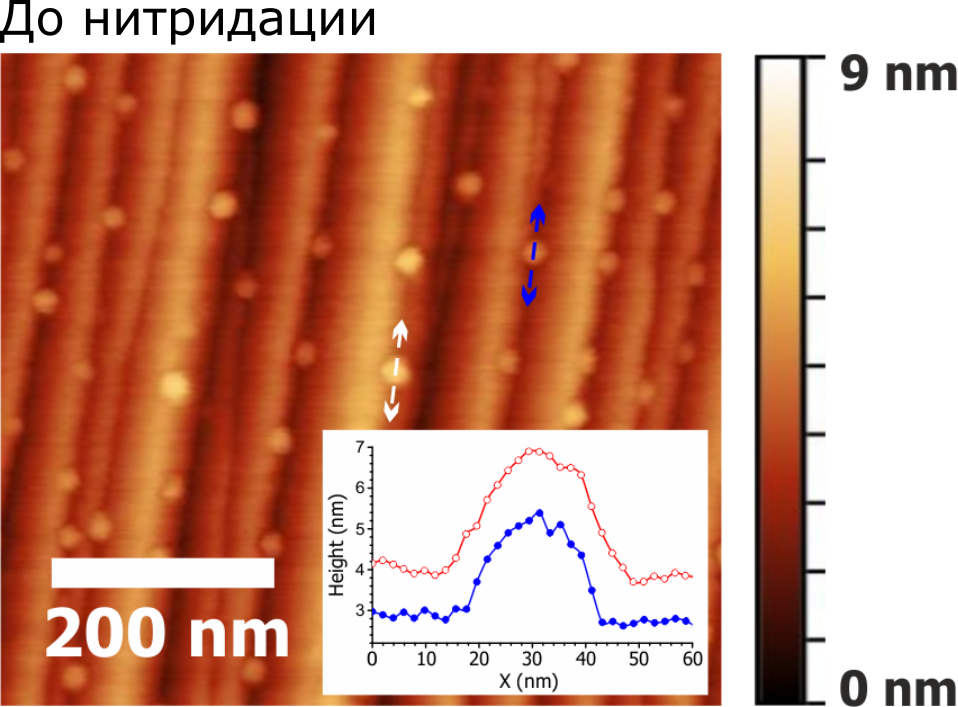
\includegraphics[width=0.45\linewidth]{Image_13_1}}
			\subcaptionbox{\label{fig:Image_13_2}}{%
		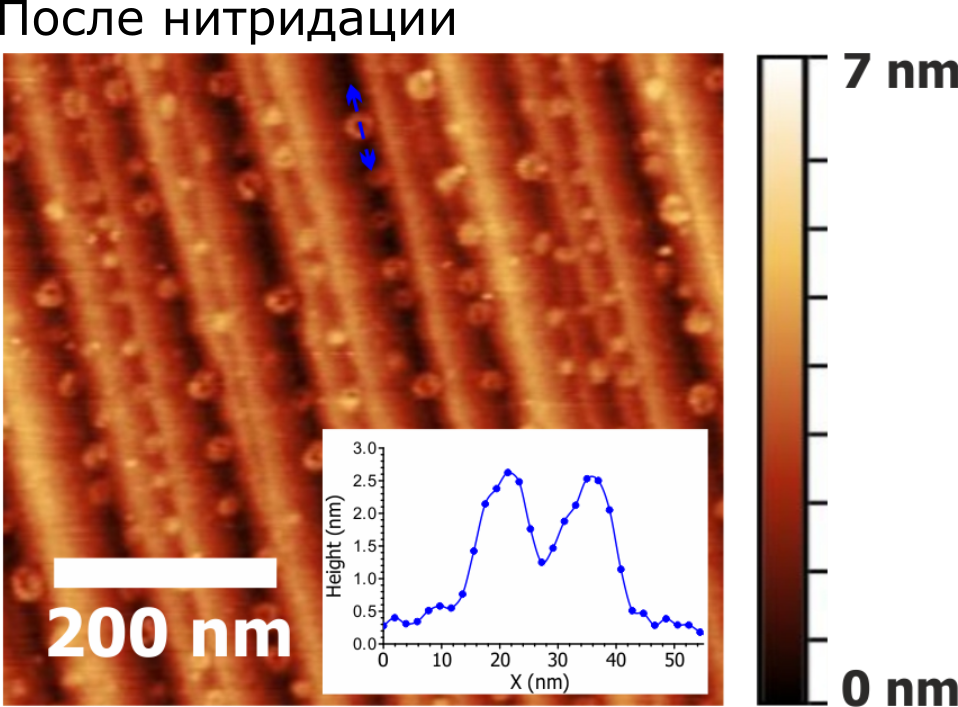
\includegraphics[width=0.45\linewidth]{Image_13_2}} } \legend{Разориентация
	поверхности 4{\textdegree} в направлении <110>. На вставках представлены
профили АСМ сканирования наноструктур} \caption{АСМ изображения поверхности Si
подложки с каплями Ga (эквивалентной толщины 1,35~монослоя) до нитридации~(а) и
после нитридации~(б)}\label{fig:Image_13} \end{figure}

Под потоком активированного азота капли кристаллизуются в кольцо высотой
1--2~\si{\nano\meter} и глубиной центрального углубления
0,5--1~\si{\nano\meter} (см. вставки на~рис.~\cref{fig:Image_13}). Схожая
морфология может быть получена капельной эпитаксией GaAs \cite{Zhou2013} и
связана с локализованным ростом соединений
A\textsuperscript{III}B\textsuperscript{V} за счет более быстрого
зародышеобразования вдоль края капли
(см.~подраздел~\cref{subsec:ch1/sec2/sub6}). После нитридации островки обладают
меньшей высотой и повышенной поверхностной плотностью по сравнению с исходными
каплями, что указывает на продолжение диффузия Ga под потоком активного азота.

Исследование ПЭМ не показало травление подложки галлием
(см.~раздел~\cref{sec:ch3/sec4}). Морфология поверхности с нитридированными
нанокольцами не изменилась после воздействия водного раствора соляной кислоты,
что указывает на отсутствие металлического Ga или эвтектического раствора Si-Ga
на поверхности после нитридации.

\section{Кристаллографические ориентации триподов}\label{sec:ch3/sec3}

Синтез GaN ННК на подложке с нитридированными каплями Ga может приводить к
формированию дополнительного массива наноструктур~--- ориентированных
наноостровков GaN в форме трипода (см.~рис.~\cref{fig:Image_14_12}).  Триподы
образованы тремя вытянутыми ветвями, расположенными под углом 120{\textdegree}
друг к другу. По отношению к базовому срезу подложки можно определить
эпитаксиальную ориентацию триподов к решётке Si: триподы имеют предпочтительную
ориентацию в плоскости подложки с выравниванием ветвей вдоль
кристаллографических направлений <\(1\overline{1}0\)>\textsubscript{Si},
<\(11\overline{2}\)>\textsubscript{Si}, <\(12\overline{3}\)>\textsubscript{Si}.
Эти ориентации показаны на рисунке~\cref{fig:Image_14_3} с указанием
пунктирными линиями кристаллических двойников, соответствующих повороту на
180{\textdegree} в плоскости подложки. Некоторые триподы имеют только одну или
две ветви.

\begin{figure}[ht] \centerfloat{ \subcaptionbox{\label{fig:Image_14_1}}{%
			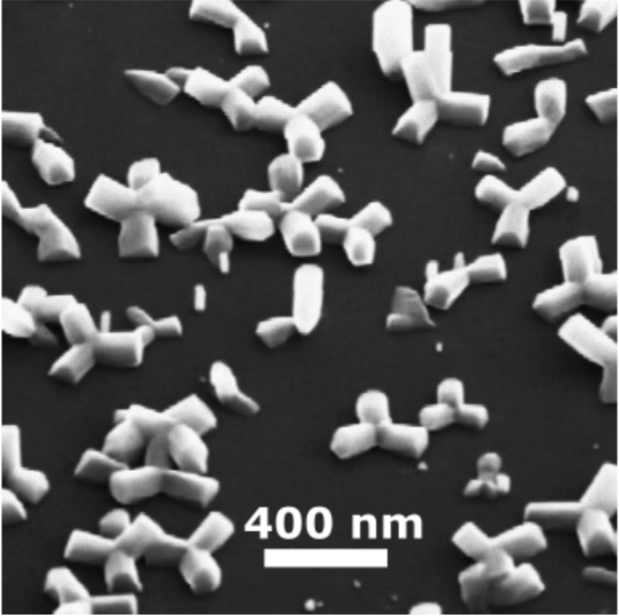
\includegraphics[width=0.4\linewidth]{Image_14_1}}
			\subcaptionbox{\label{fig:Image_14_2}}{%
		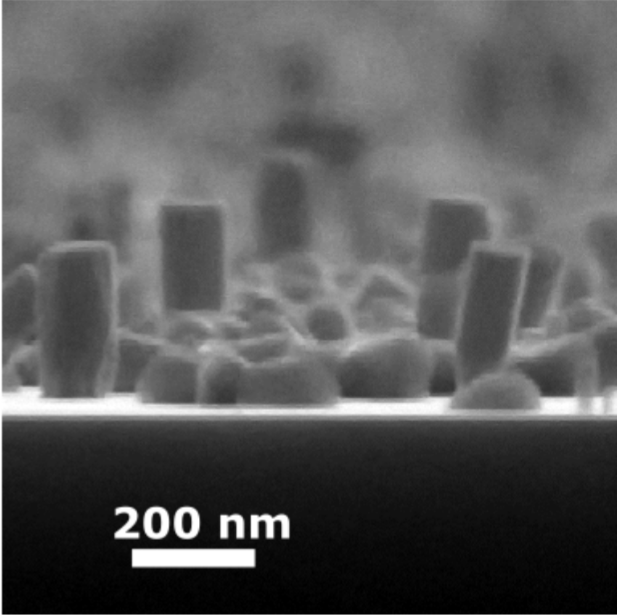
\includegraphics[width=0.4\linewidth]{Image_14_2}} } \legend{Изометрический
	вид~(а), вид сбоку~(б)} \caption{РЭМ изображения эпитаксиальных нанотриподов
	GaN}\label{fig:Image_14_12} \end{figure}

\begin{figure}[ht] \centerfloat{
	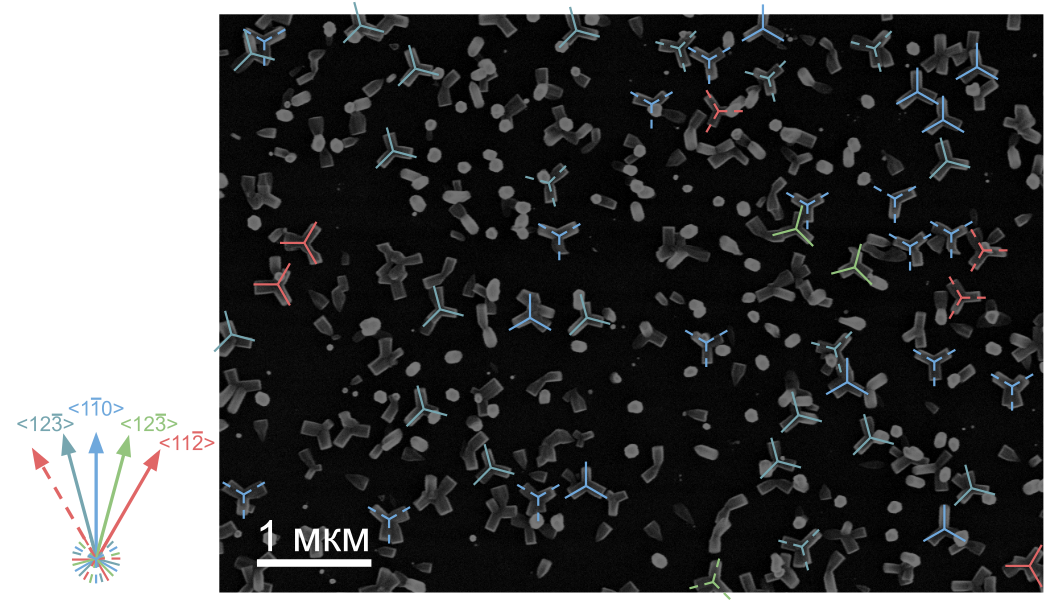
\includegraphics[width=1\linewidth]{Image_14_3} } \legend{Ориентации триподов
схематически обозначены цветными символами. Кристаллографические направления
указаны на схеме слева} \caption{РЭМ изображение эпитаксиальных нанотриподов
GaN, вид сверху}\label{fig:Image_14_3} \end{figure}

Формирование подобных GaN триподов уже было исследовано в ряде работ: на
c-плоскости Al\textsubscript{2}O\textsubscript{3} методом хлорид-гидридной
газофазной эпитаксии \cite{Lee2010}, на наноколоннах GaN методом ПА-МПЭ
\cite{Wang2017}, на алмазной подложке методом селективной эпитаксии
\cite{Schuster2015}.

\section{Исследование кристаллической структуры методом
ПЭМ}\label{sec:ch3/sec4}

На подложке с поверхностной реконструкцией Si\((111)6,3\)\(\times\)\(6,3 -
\text{Ga}\) синтезирован массив наноструктур (см.~раздел~\cref{sec:ch3/sec1}).
На гетероинтерфейсе GaN/Si (см.~рис.~\cref{fig:Image_15_1}) наблюдается
аморфный слой толщиной \(\approx 1,5\)~\si{\nano\meter}. Данный слой может быть
аморфным SiN\textsubscript{x}, который может формироваться в процессе
нитридации затравочных капель при взаимодействии поверхности Si с активным
азотом. У данного процеса существует несколько механизмов: до насыщения азотом
и образования зародыша капли Ga мигрируют по поверхности Si, которая уже
провзаимодействовала с потоком азота; в процессе насыщения капли Ga часть
растворенных молекул азота взаимодействует с поверхностью подложки под каплей;
адомы азота дифундируют в приповерхностном слое Si \cite{Rawdanowicz2004}.

\begin{figure}[ht] \centerfloat{ \subcaptionbox{\label{fig:Image_15_1}}{%
			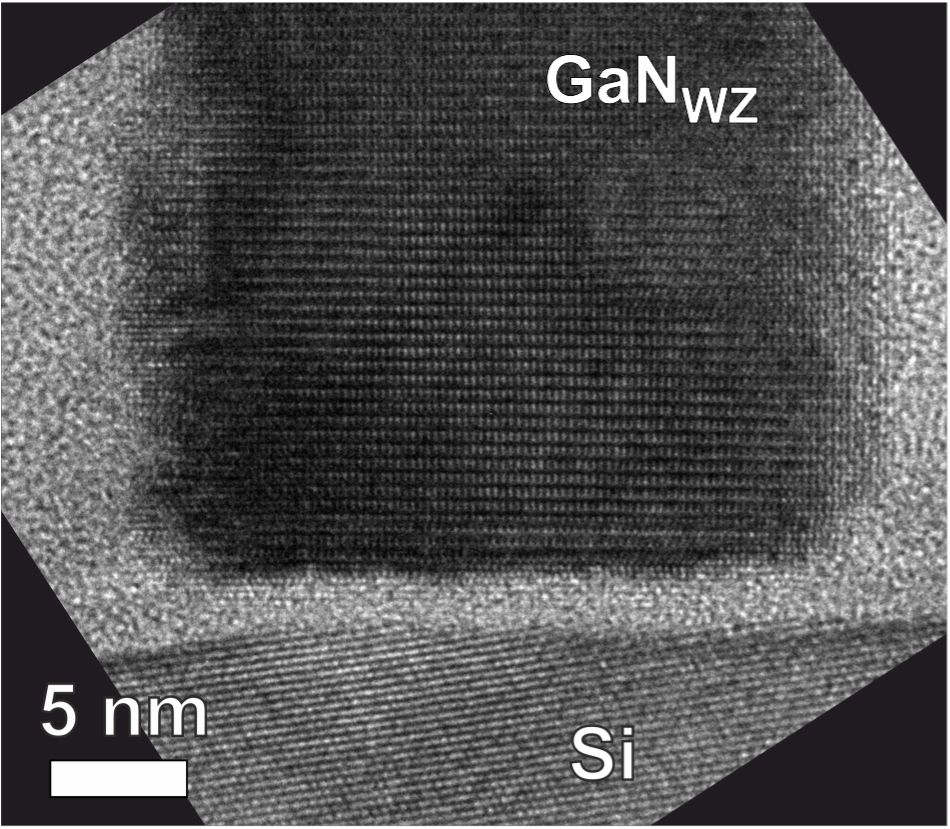
\includegraphics[height=7cm]{Image_15_1}}
			\subcaptionbox{\label{fig:Image_15_2}}{%
		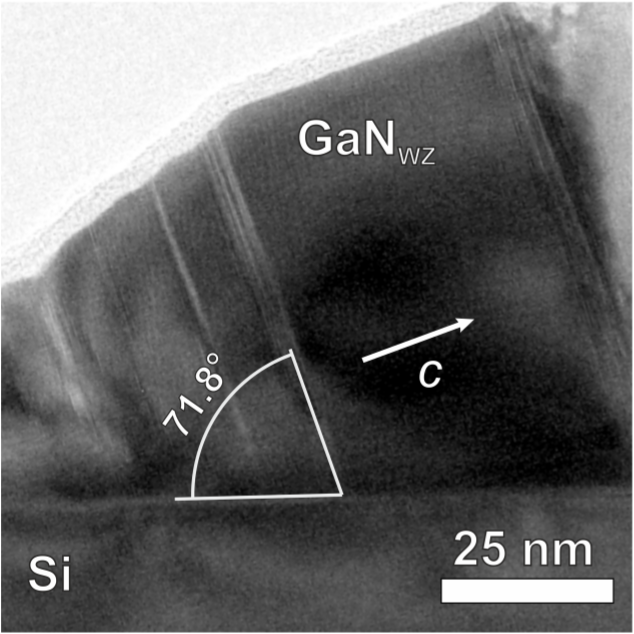
\includegraphics[height=7cm]{Image_15_2}} } \caption{ВРЭМ изображение
	гетероинтерфейса вертикального ННК GaN с подложкой Si(111)~(а), ПЭМ
изображение ветви трипода GaN на подложке Si(111)~(б)}\label{fig:Image_15}
\end{figure}

Согласно работе \cite{Lee2010}, формирование нанотриподов GaN начинается с
образования ZB наноостровка с последующим зарождением и ростом в плоскости
подложки WZ наностержней на его \{111\} фасетках. Изучение триподов методом ПЭМ
затруднено формированием муарового контраста от наложения решёток ветви и ядра,
поэтому выводы о структуре ядра триподов были сделаны на основе изучения схожих
объектов массива.

При изучении ПЭМ изображений образца были обнаружены наклонный ННК и ветвь
нанотрипода с общим ядром (см.~рис.~\cref{fig:Image_16}). На картинах
электронной микродифракции этих структур были видны рефлексы только WZ
структуры GaN, так как интенсивность рассеяния на ядре наночастицы была
недостаточной для регистрации из-за ее малого объема.

Упаковка кристаллической решётки WZ и ZB была различима на изображениях ВРЭМ с
ориентацией образца вдоль оси зоны
\([\overline{1}2\overline{1}0]\)\textsubscript{WZ GaN}. Изображения быстрого
преобразования Фурье (БПФ) от отмеченных пунктирными квадратами областей
наноструктуры с различными упаковками представлены
на~рис.~\cref{fig:Image_16_2}. Расчетные сечения обратного пространства WZ и ZB
структур с соответствующими осями зон
\([\overline{1}2\overline{1}0]\)\textsubscript{WZ GaN} и
\([\overline{11}0]\)\textsubscript{ZB GaN} отмечены на изображениях БПФ
оранжевыми и белыми пунктирными кружками соответственно.

\begin{figure}[ht] \centerfloat{ \subcaptionbox{\label{fig:Image_16_1}}{%
			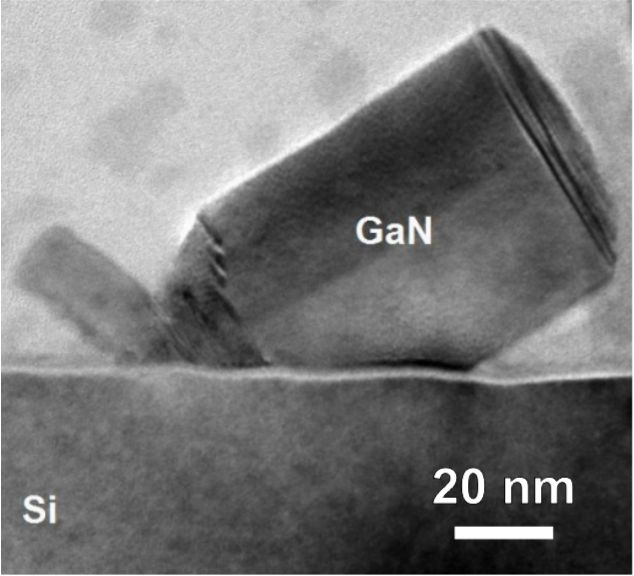
\includegraphics[height=8cm]{Image_16_1}}
			\subcaptionbox{\label{fig:Image_16_2}}{%
			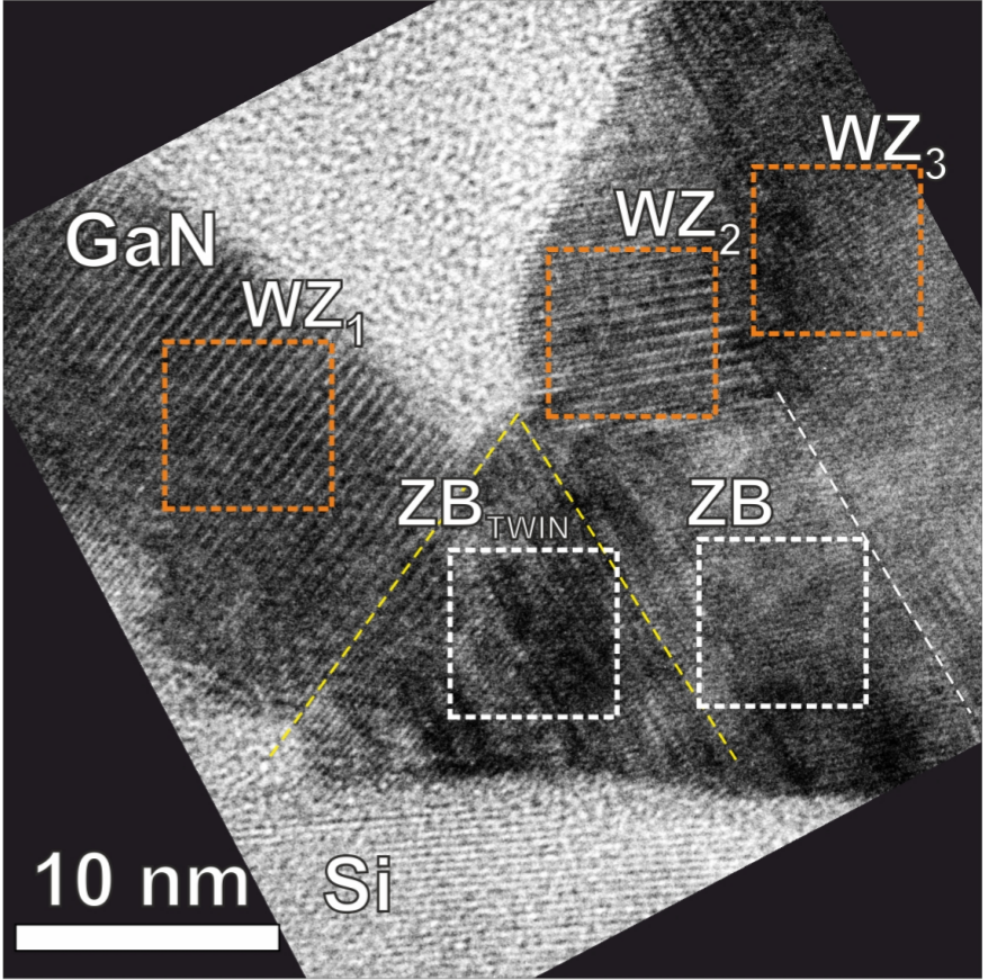
\includegraphics[height=8cm]{Image_16_2}}

	\subcaptionbox{\label{fig:Image_16_3}}{%
		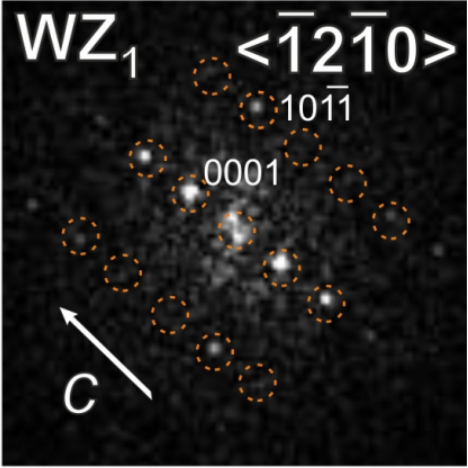
\includegraphics[width=0.19\linewidth]{Image_16_3}}
		\subcaptionbox{\label{fig:Image_16_4}}{%
			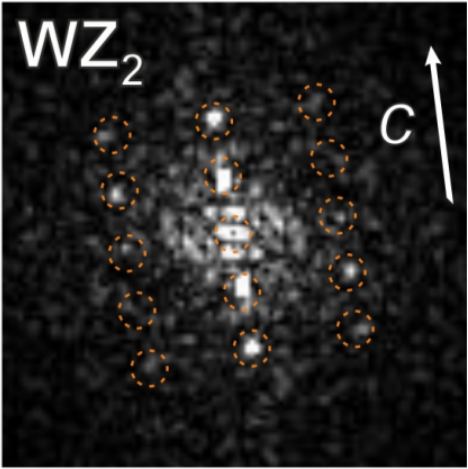
\includegraphics[width=0.19\linewidth]{Image_16_4}}
			\subcaptionbox{\label{fig:Image_16_5}}{%
			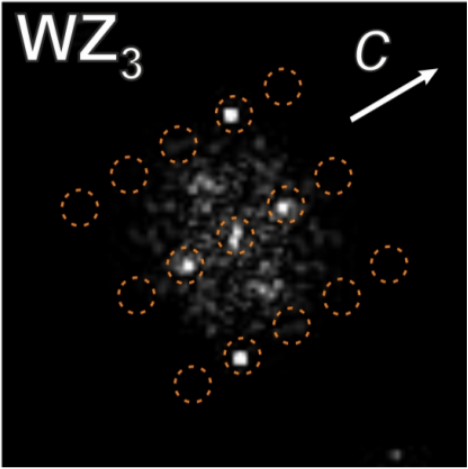
\includegraphics[width=0.19\linewidth]{Image_16_5}}
			\subcaptionbox{\label{fig:Image_16_6}}{%
				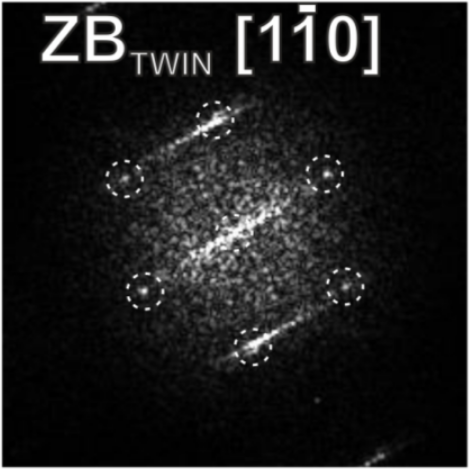
\includegraphics[width=0.19\linewidth]{Image_16_6}}
				\subcaptionbox{\label{fig:Image_16_7}}{%
				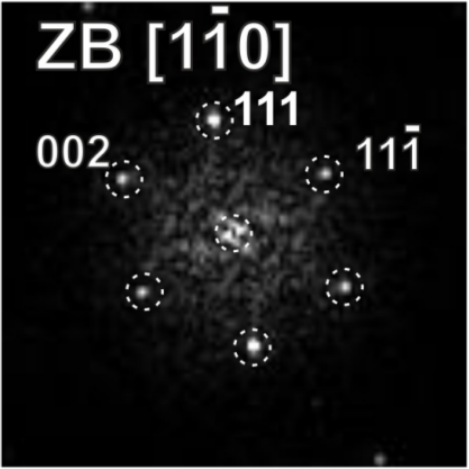
\includegraphics[width=0.19\linewidth]{Image_16_7}} }
				\caption{Микроснимок ПЭМ наклонного ННК и ветви трипода GaN с общим
				центром~(а). Вид крупным планом ВРЭМ~(б) с соответствующими
			изображениями БПФ от областей, отмеченных пунктирными
		квадратами~(в\,--\,ж)}\label{fig:Image_16} \end{figure}

В результате БПФ анализа отчётливо видно отличие кристаллической структуры
основания от ветви и наклонного ННК: наиболее заметное отличие~---
периодичность и симметрия БПФ образа, соответствующая гексагональной и
кубической последовательности укладки плотно упакованных плоскостей
\cite{Jo2018, Bayram2014}. В базовой части (отмечена
на~рис.~\cref{fig:Image_16_2} как ZB и ZB\textsubscript{twin}) периодичность
типа ABCABC{\dots} соответствует GaN со структурой ZB (вдоль <111>). Каждая из
букв A, B и C обозначает бислой атомов, состоящий из одного слоя с атомами
группы III и одного слоя с атомами группы V. У наклонного ННК и ветви
(обозначены на~рис.~\cref{fig:Image_16_2} как WZ\textsubscript{1},
WZ\textsubscript{2}, WZ\textsubscript{3}) периодичность типа ABAB{\dots}
соответствует GaN со структурой WZ (вдоль <0001>) \cite{Kriegner2011}.

Таким образом, WZ триподы и наклонные ННК имеют в основании ZB наноостровок. В
простейшем случае он имеет тетраэдрическую форму с гранями
\{111\}\textsubscript{ZB GaN}, плоскость (111)\textsubscript{ZB GaN} которых
ориентирована параллельно Si(111). Такое ZB ядро служит центром
зародышеобразования трипода или наклоненного ННК. Вертикальные ННК
(см.~рис.~\cref{fig:Image_15_1}) не имеют в основании затравочных островков.

Зарождение метастабильной ZB структуры GaN связывают с низкой температурой
роста или избытком Ga \cite{Shi2006, Romano1997}. Аналогичное образование ННК
InAs с метастабильной WZ структурой объясняют размерными эффектами
\cite{Johansson2010}.

Яркие полосы вдоль направления \([11\overline{1}]\) на БПФ образе области
ZB\textsubscript{twin} (см.~рис.~\cref{fig:Image_16_2}) свидетельствуют о
наличии планарных дефектов в плоскости перпендикулярной направлению тяжей.
Главным образом планарные дефекты~--- это кристаллические двойникования,
соответствующие повороту на 180{\textdegree} вокруг направления
\([11\overline{1}]\)\textsubscript{ZB GaN}. Подобное двойникование может
происходить вокруг любого направления <111> \cite{Suturin2017} и приводить к
формированию двойниковой \{111\}\textsubscript{ZB GaN} грани внутри одного ZB
островка (см.~подраздел~\cref{subsec:ch1/sec2/sub5}). Ориентация таких граней
определяет направление роста наклонных ННК.

Линейные контрастные особенности на ПЭМ изображениях ветвей трипода
на~рисунках~\cref{fig:Image_16_1}~и~\cref{fig:Image_15_2} связаны с двумерными
дефектами, перпендикулярными направлению (0001)\textsubscript{WZ GaN}
(см.~подраздел~\cref{subsec:ch1/sec2/sub5}). Преимущественно это дефекты
упаковки.

Угол между плоскостью Si(111) и (0001)\textsubscript{WZ GaN} ветви трипода,
изображенном на~рис.~\cref{fig:Image_15_2} составляет \(72\si{\degree} \pm
1\si{\degree}\), что соответствует значению угла между плоскостями
(0001)\textsubscript{WZ GaN} и \((11\overline{2}1)\)\textsubscript{WZ GaN}
(72,92\textdegree) \cite{Wang2016}. Таким образом, кристаллографическая
плоскость \((11\overline{2}1)\)\textsubscript{WZ GaN} ветвей триподов GaN
параллельна поверхности подложки Si(111).

На другом образце с эквивалентной толщиной затравочного Ga в 2~монослоя
наблюдались двойные наклонные ННК (см.~рис.~\cref{fig:Image_18}). На
изображении ВРЭМ (см.~рис.~\cref{fig:Image_18_2}) наблюдается общее ZB ядро
двойных наклонных ННК. Из БПФ образов заметно, что в отличии от предыдущего
случая, грань (001)\textsubscript{ZB GaN} ядра ориентирована перпендикулярно
плоскости подложки Si(111). Подобная морфология наблюдалась в работе
\cite{Wang2017}.

\{111\}\textsubscript{ZB GaN} ядра служат центрами зародышеобразования WZ ННК.
Угол между осями сросшихся ННК \(\approx 116\){\textdegree} (угол между [111] и
\([\overline{111}]\) составляет 109,47\textdegree), что указывает на
формирование \([\overline{1}103]\)\textsubscript{WZ GaN} плоскости сращивания,
а не ожидаемой \([\overline{3}308]\)\textsubscript{WZ GaN}.

Подводя итог, триподы и наклонные ННК имеют в основании ZB ядро, а их
морфология зависит от кристаллографической ориентации и возможных
кристаллических двойникований ядра.

\begin{figure}[ht] \centerfloat{ \subcaptionbox{\label{fig:Image_18_1}}{%
			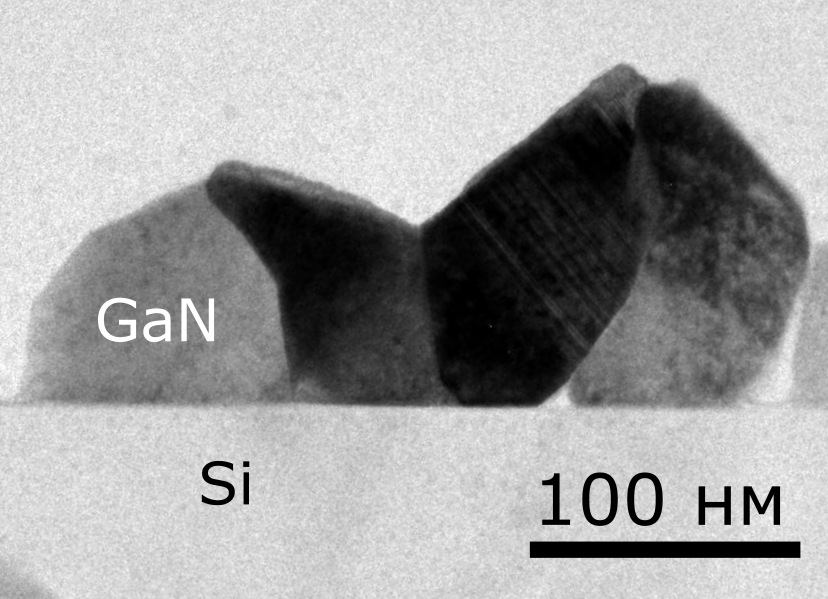
\includegraphics[height=7cm]{Image_18_1}}
			\subcaptionbox{\label{fig:Image_18_2}}{%
			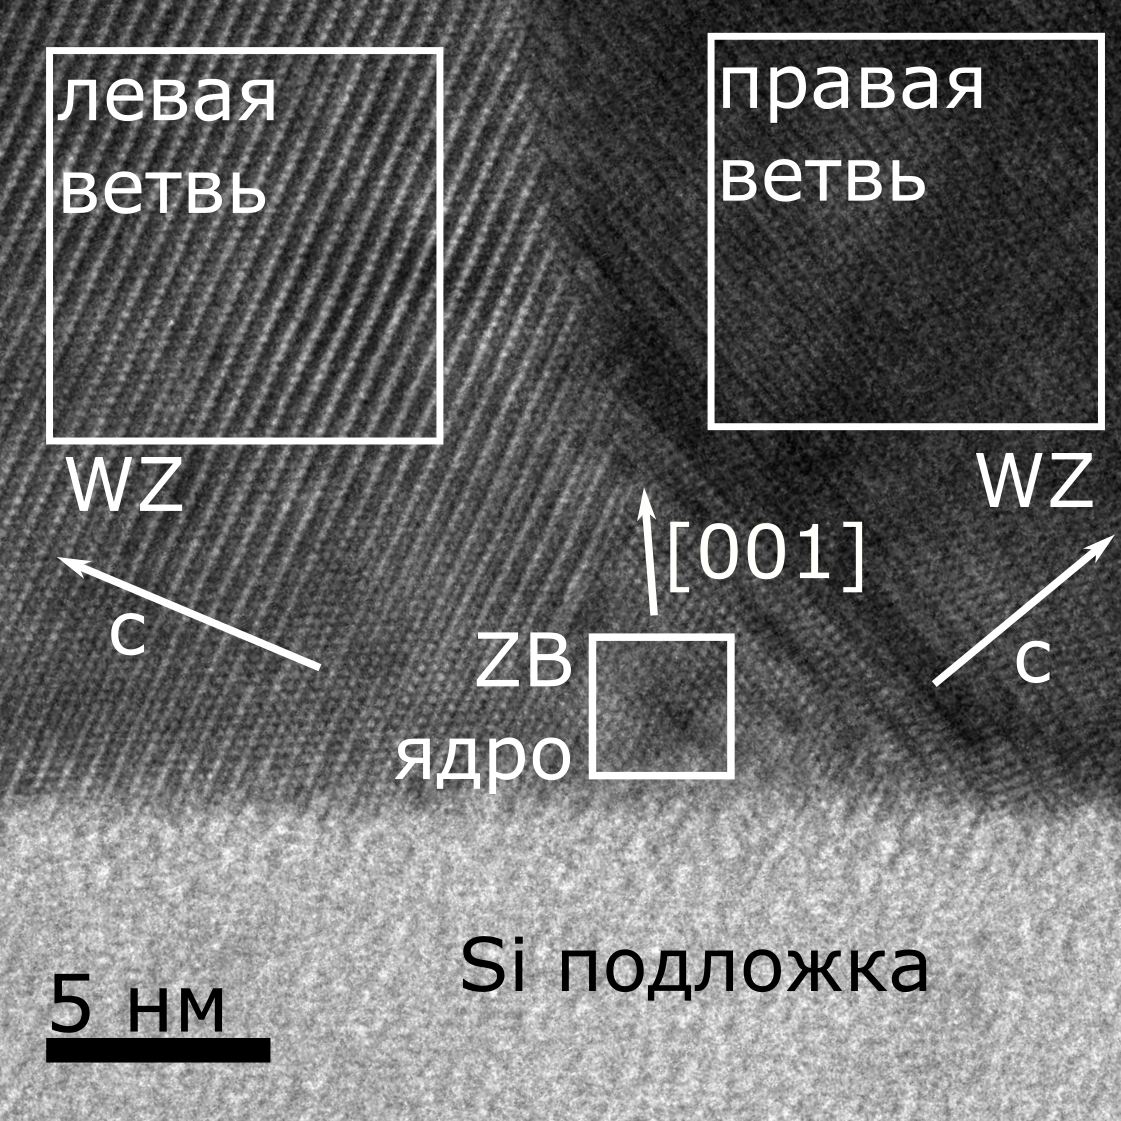
\includegraphics[height=7cm]{Image_18_2}}

		\subcaptionbox{\label{fig:Image_18_3}}{%
			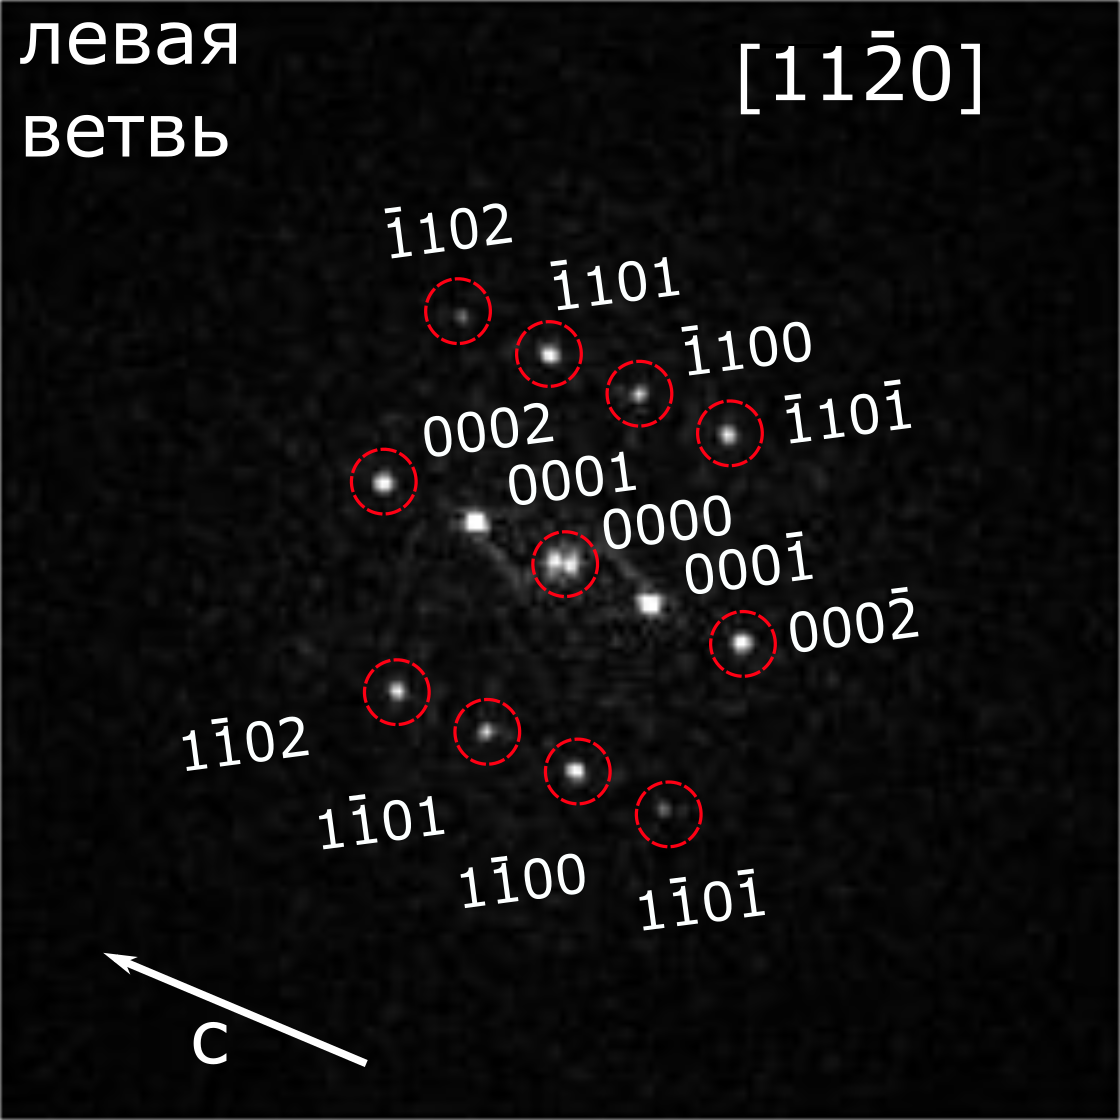
\includegraphics[width=0.31\linewidth]{Image_18_3}}
			\subcaptionbox{\label{fig:Image_18_4}}{%
				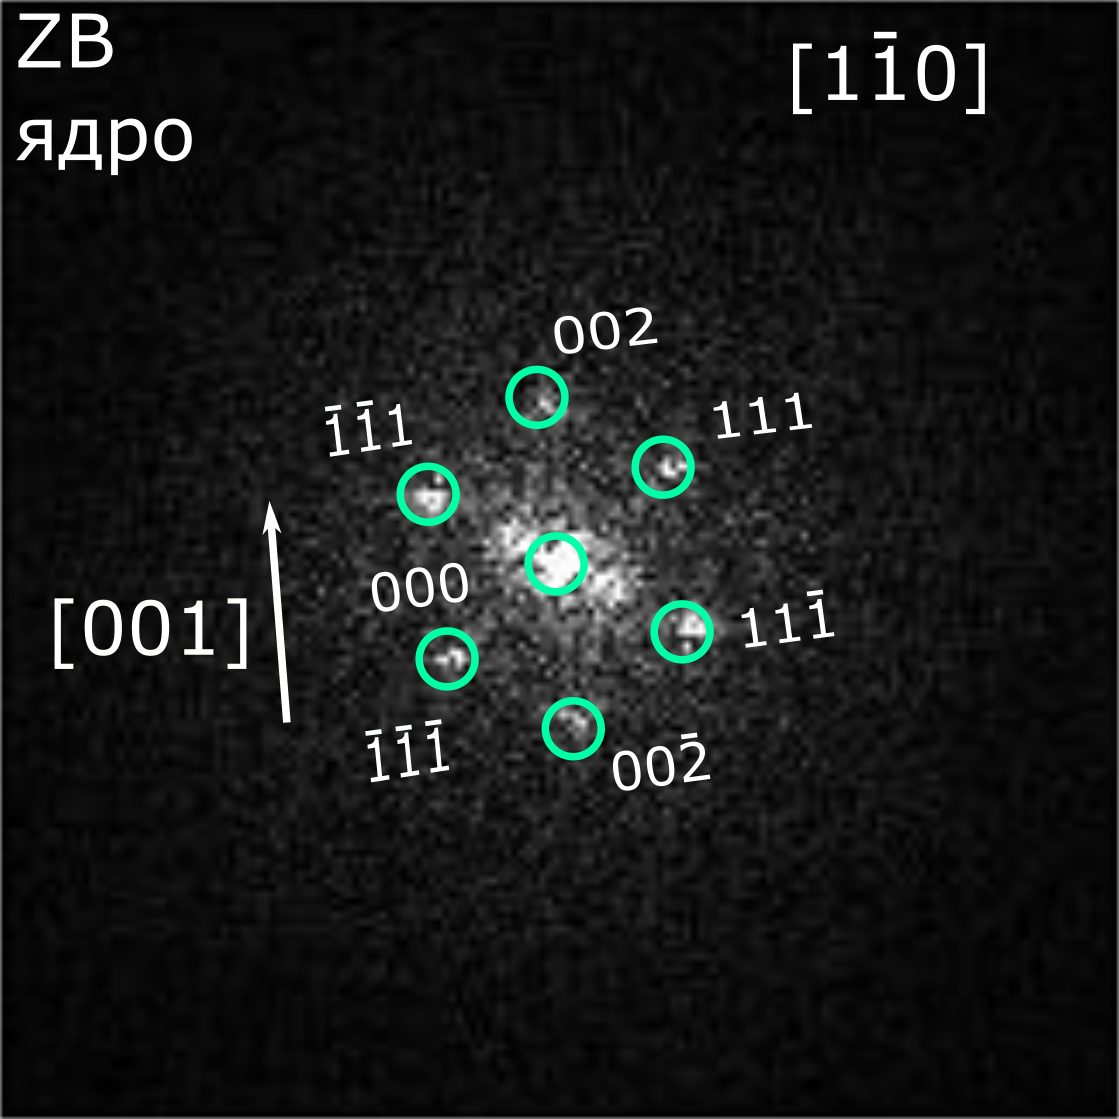
\includegraphics[width=0.31\linewidth]{Image_18_4}}
				\subcaptionbox{\label{fig:Image_18_5}}{%
				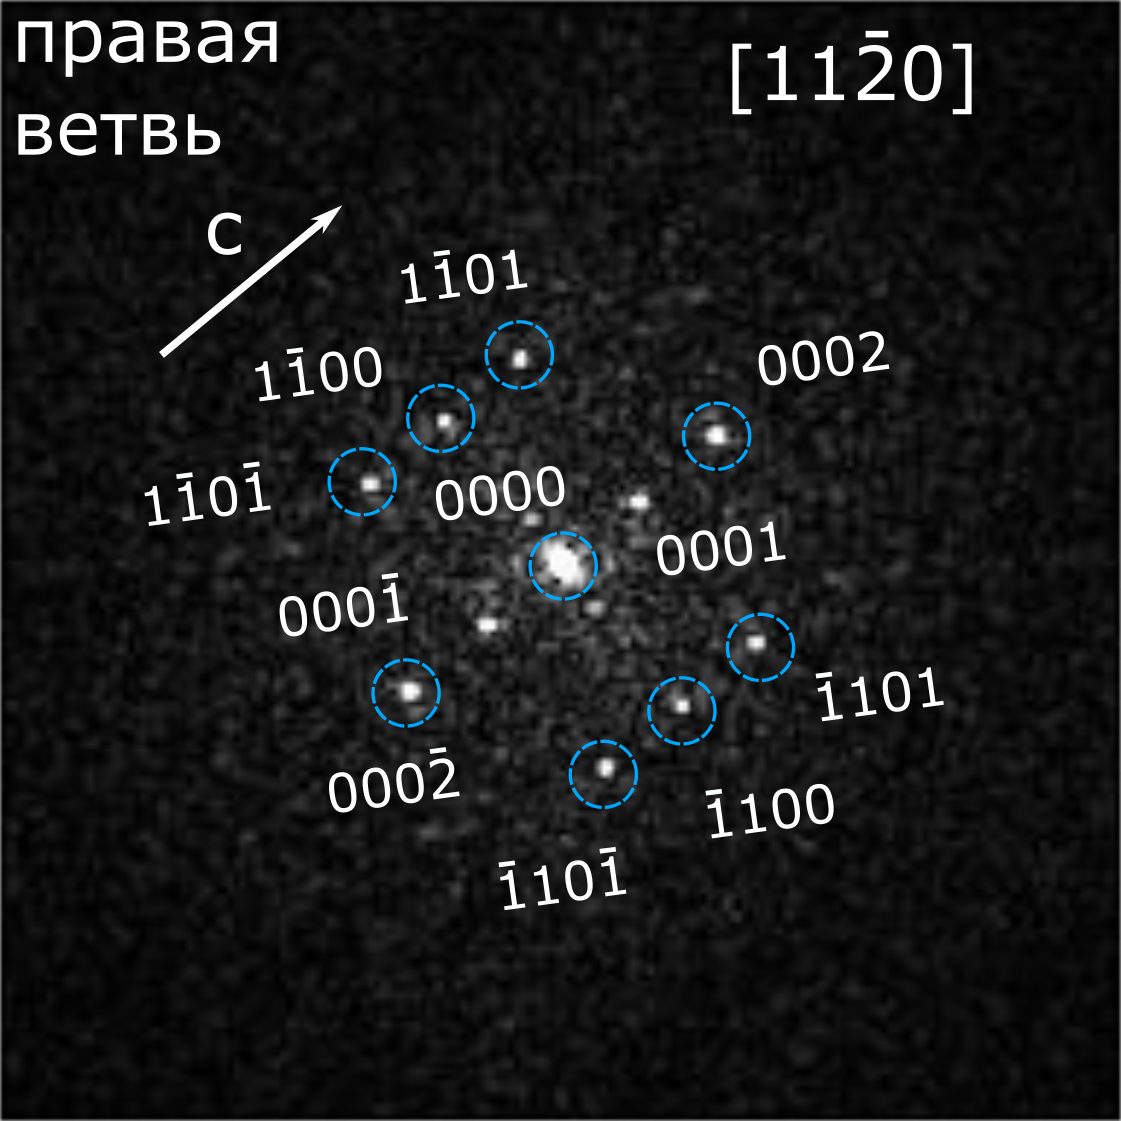
\includegraphics[width=0.31\linewidth]{Image_18_5}} } \caption{ПЭМ
			изображение наклонных ННК GaN с общим ядром~(а). Вид крупным планом
		ВРЭМ~(б) с соответствующими изображениями БПФ от отмеченных квадратами
	областей~(в\,--\,д)}\label{fig:Image_18} \end{figure}

\section{Исследование ФЛ триподов}\label{sec:ch3/sec5}

Для исследования ФЛ был выбран образец с высокой поверхностной плотностью
триподов \((\approx 20~\si{\micro\meter^{-2}})\). Измерения проводились при
температуре 10~\si{\kelvin} с возбуждением на длине волны 325~\si{\nano\meter}
непрерывным HeCd лазером. Типичный спектр ФЛ ансамбля нанотриподов GaN
(см.~рис.~\cref{fig:Image_19}) имеет три полосы: A (\(\approx
3,48\)~\si{\electronvolt}), B (\(\approx 3,43\)~\si{\electronvolt}) и C
(\(\approx 3,25\)~\si{\electronvolt)}.

Полоса A характерна для объемного GaN со структурой WZ и соответствует
излучению вблизи края поглощения, что может быть связано со связанными на
нейтральном доноре экситонами \cite{Bolshakov2018, Richter2008, Agekyan2013}.

Полоса B может быть связана со структурными дефектами \cite{Calleja2000}, в
частности с наблюдаемыми дефектами упаковки в триподах
(см.~рис.~\cref{fig:Image_15_2}) \cite{Albrecht1997, Paskov2005}. В
Ni-каталитических ННК подобный пик вызван примесями Ni или наличием Ga вакансий
в структуре \cite{Yoo2006}.

Широкая полоса C может быть вызвана включениями ZB в GaN, так как ZB GaN при
низких температурах излучает вблизи края поглощения с энергией \(\approx
3,27\)~\si{\electronvolt} \cite{Jacobs2007}.

\begin{figure}[ht] \centerfloat{
	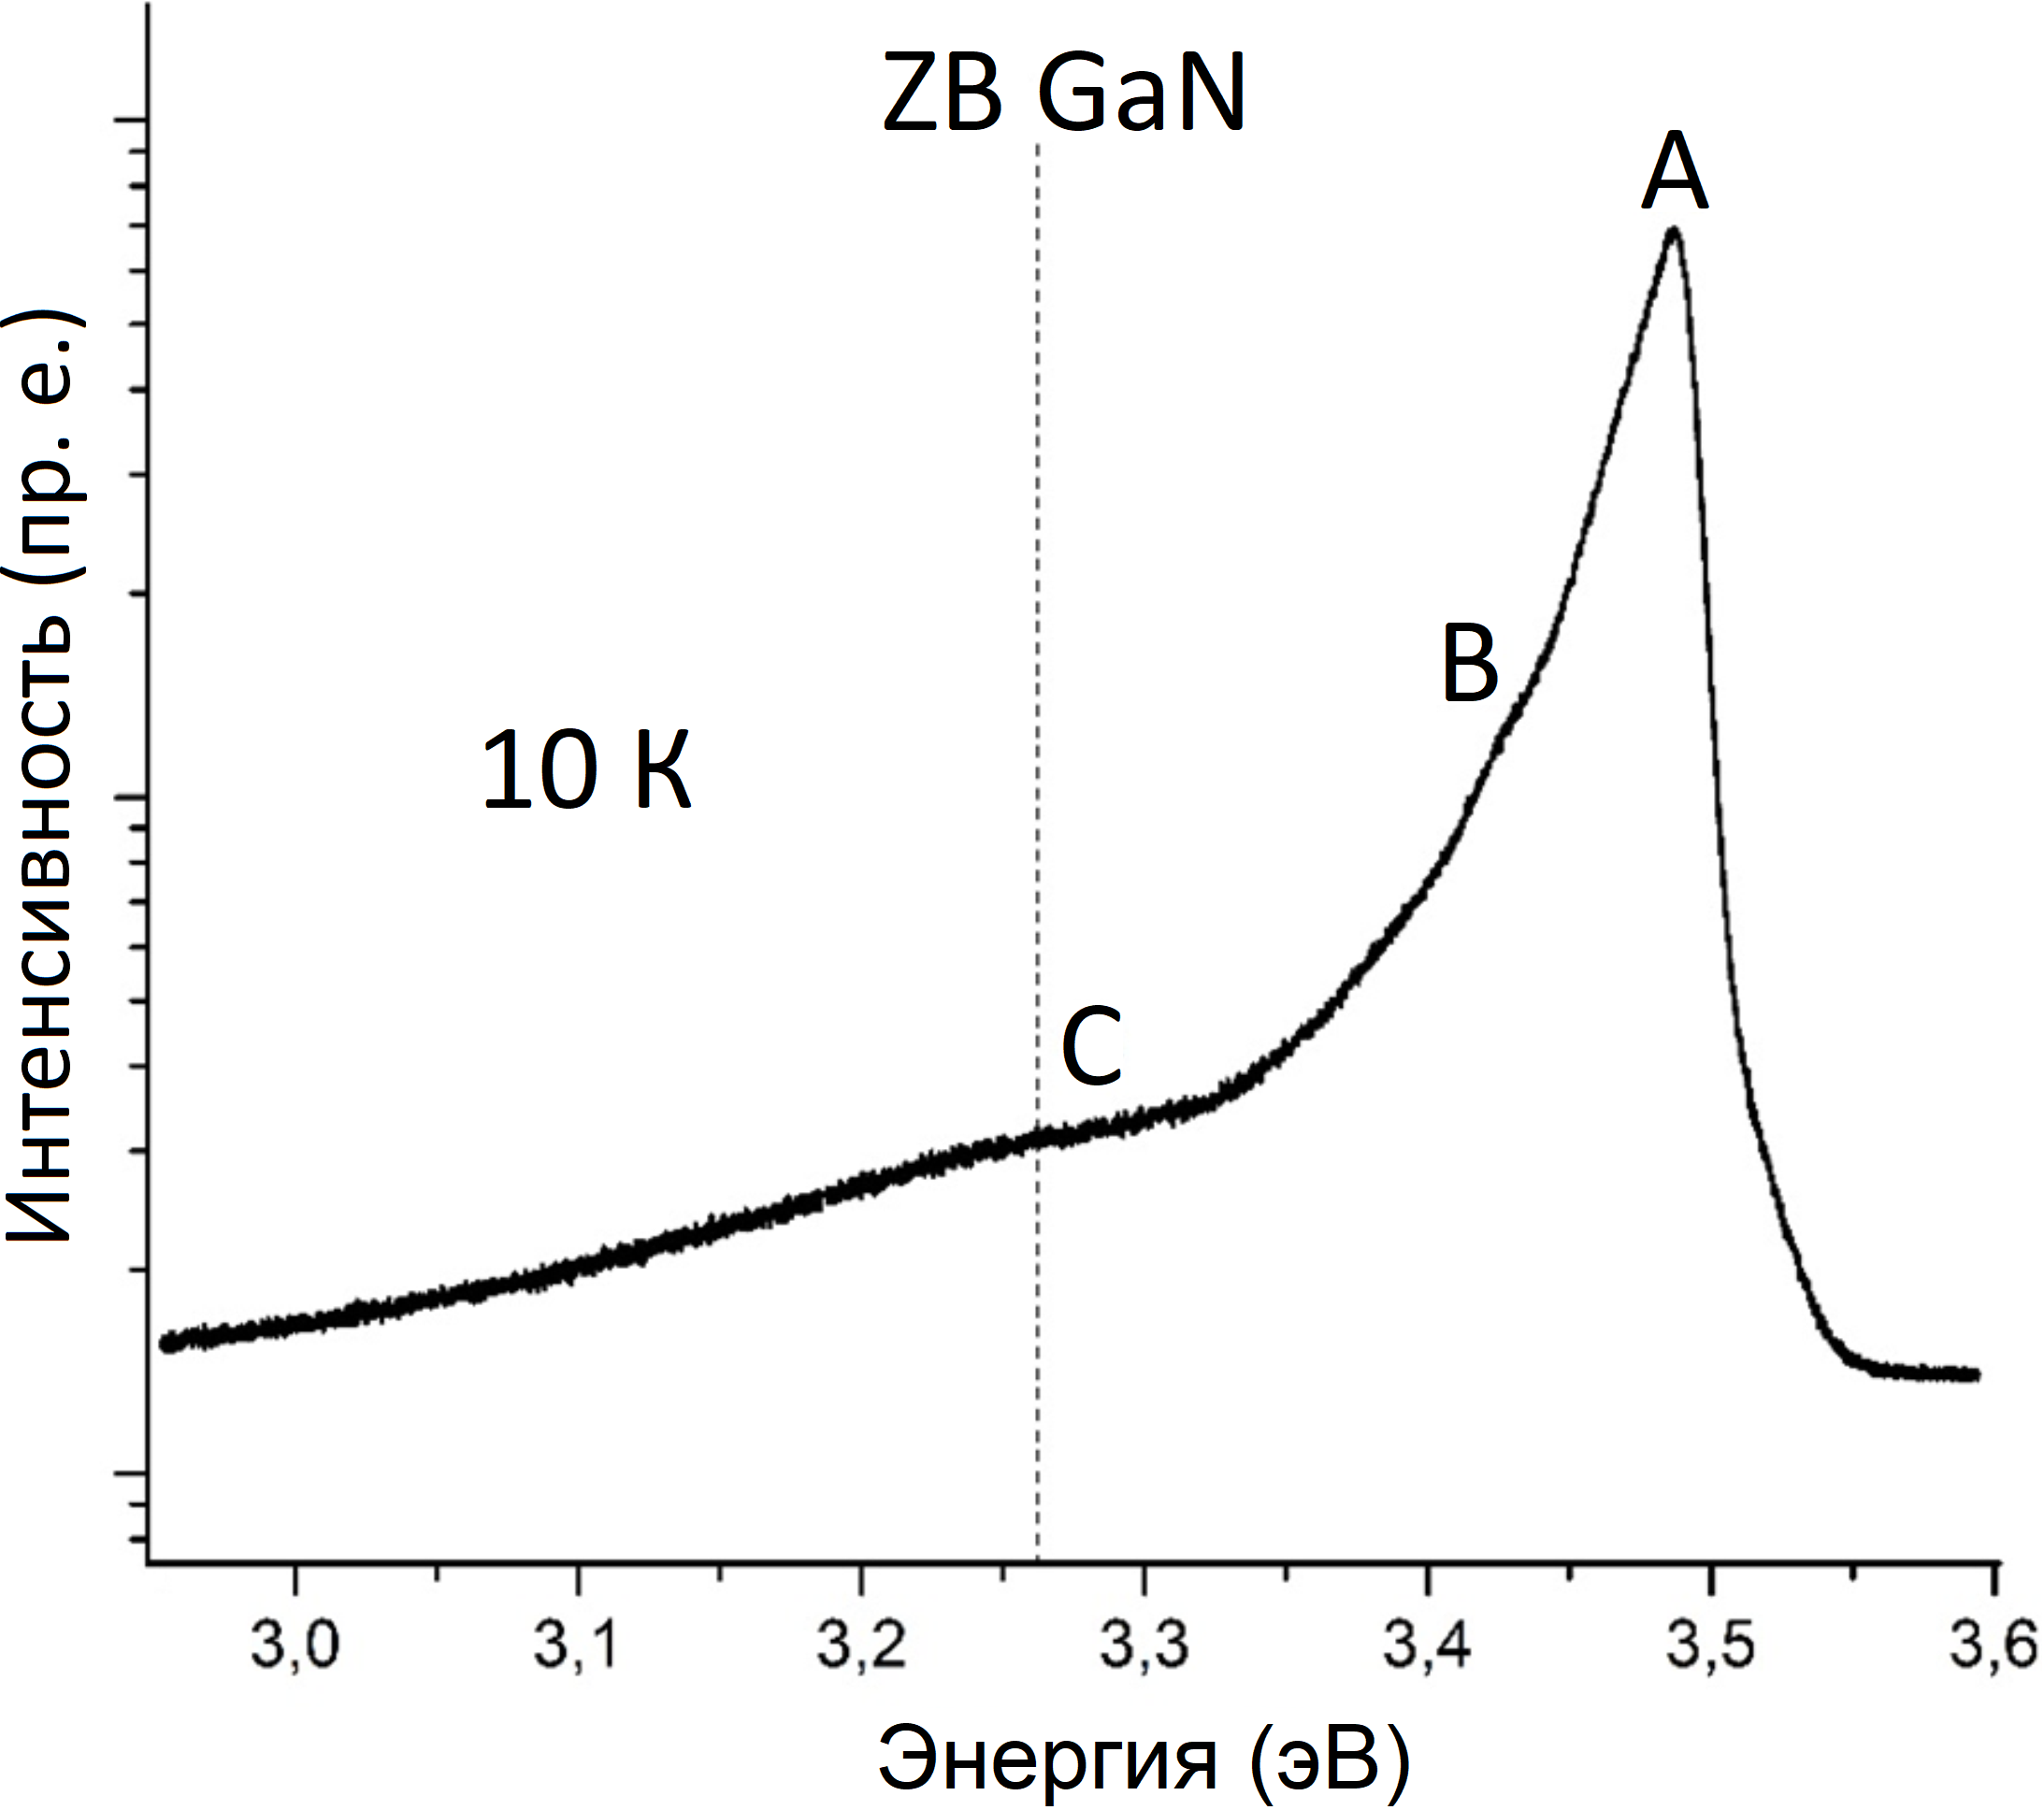
\includegraphics[width=0.5\linewidth]{Image_19} } \legend{Морфология
поверхности образца изображена на~рисунке~\cref{fig:Image_25_1}, спектр снят
при температуре 10~\si{\kelvin}} \caption{Низкотемпературный спектр ФЛ массива
эпитаксиальных триподов GaN с высокой поверхностной
плотностью}\label{fig:Image_19} \end{figure}

\section{Влияние ростовых условий на морфологию
наноструктур}\label{sec:ch3/sec6}

\subsection{Влияние эквивалентной толщины затравочных
капель}\label{subsec:ch3/sec6/sub1}

Наноструктуры для анализа влияния эквивалентной толщины затравочных капель на
морфологию были синтезированы наноструктуры при следующих условиях роста: ЭДП
Ga \(1 \cdot 10^{-8}\)~\si{\torr}, расход азота
0,4~\si{\centi\meter^3\per\minute} и мощность плазменного источника
500~\si{\watt}.

Из сравнения образцов с нитридированными каплями различной эквивалентной
толщины (см.~рис.~\cref{fig:Image_20}) видно, что в исследуемом диапазоне
увеличение количества предварительно осажденного Ga повышает плотность
затравочных островков GaN, но слабо влияет на их латеральный размер и
морфологию.

\begin{figure}[ht] \centerfloat{ \subcaptionbox{\label{fig:Image_20_1}}{%
			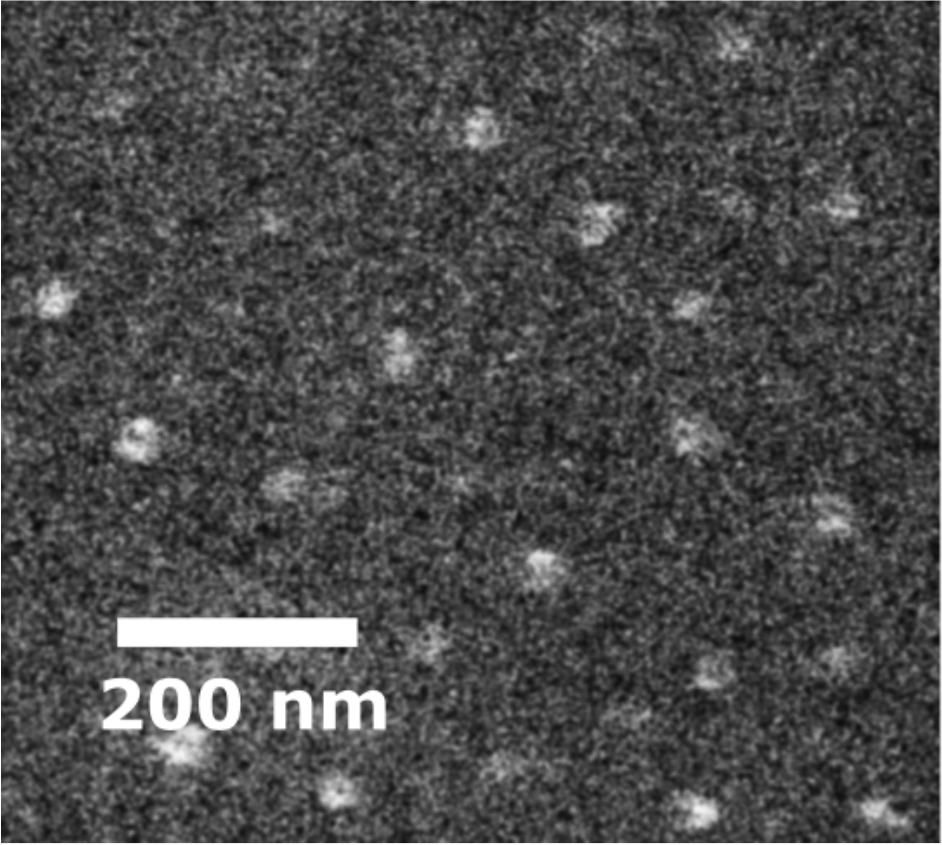
\includegraphics[width=0.25\linewidth]{Image_20_1}}
			\subcaptionbox{\label{fig:Image_20_2}}{%
		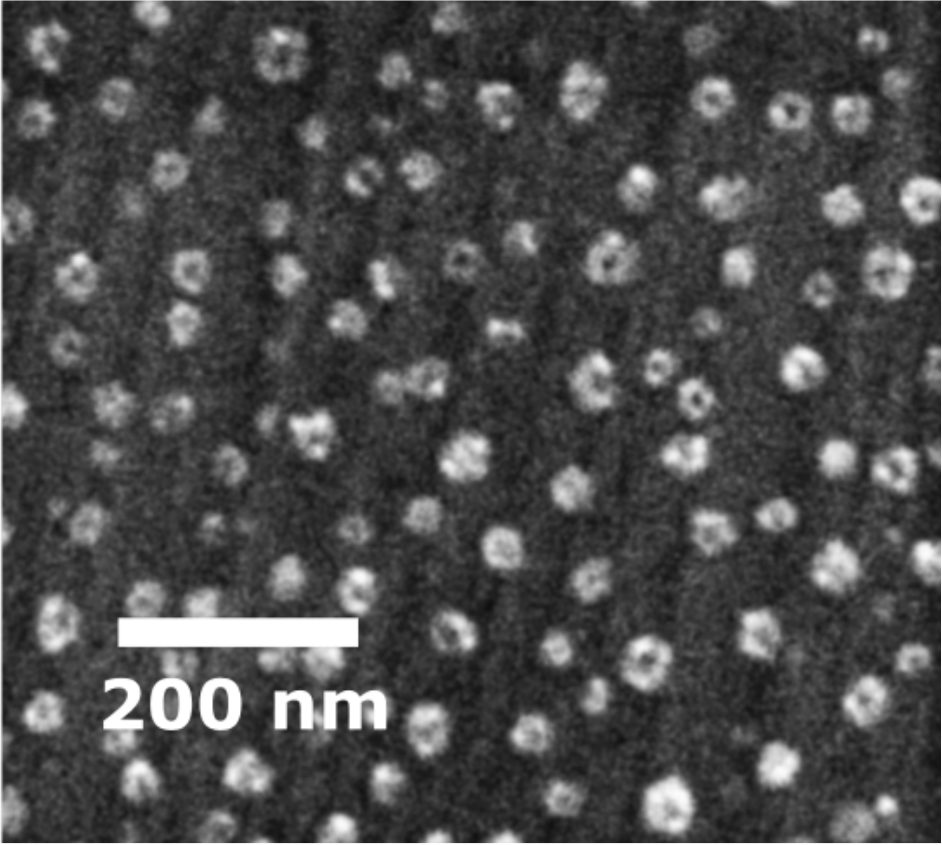
\includegraphics[width=0.25\linewidth]{Image_20_2}} } \legend{Эквивалентная
	толщиной капель Ga 1,35~(а) и 2~монослоя~(б)} \caption{РЭМ изображения
затравочных островков GaN, выращенных методом капельной эпитаксии с различной
эквивалентной толщиной капель Ga}\label{fig:Image_20} \end{figure}

Затравка Ga с эквивалентной толщиной менее 1~монослоя образует поверхностную
реконструкцию (см.~подраздел~\cref{subsec:ch2/sec1/sub2}), поэтому после
нитридации ZB островки не образуются. Следовательно, формирование триподов
подавляется, образуются исключительно ННК (см.~рис.~\cref{fig:Image_21}).

\begin{figure}[ht] \centerfloat{ \subcaptionbox{\label{fig:Image_21_1}}{%
			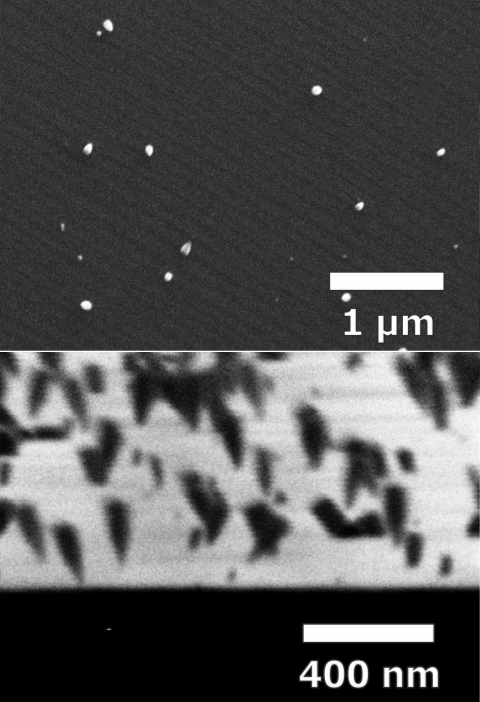
\includegraphics[width=0.25\linewidth]{Image_21_1}}
			\subcaptionbox{\label{fig:Image_21_2}}{%
		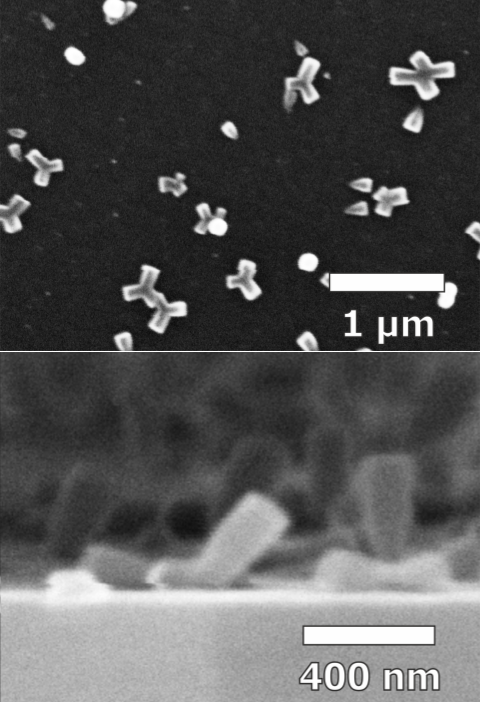
\includegraphics[width=0.25\linewidth]{Image_21_2}} } \legend{Эквивалентная
	толщина Ga 0,7~(а) и 2~монослоя~(б)} \caption{РЭМ изображения морфологии
наноструктур GaN, синтезированных на затравочных островках различной
эквивалентной толщины}\label{fig:Image_21} \end{figure}

Увеличение эквивалентной толщины затравки в диапазоне 0,7--1,4~монослоя
приводит к увеличению поверхностной плотности затравочных островков, а вместе с
тем увеличивает плотность и эквивалентную толщину синтезированных нанотриподов
(см.~рис.~\cref{fig:Image_22}).

\begin{figure}[ht] \centerfloat{ \subcaptionbox{\label{fig:Image_22_1}}{%
			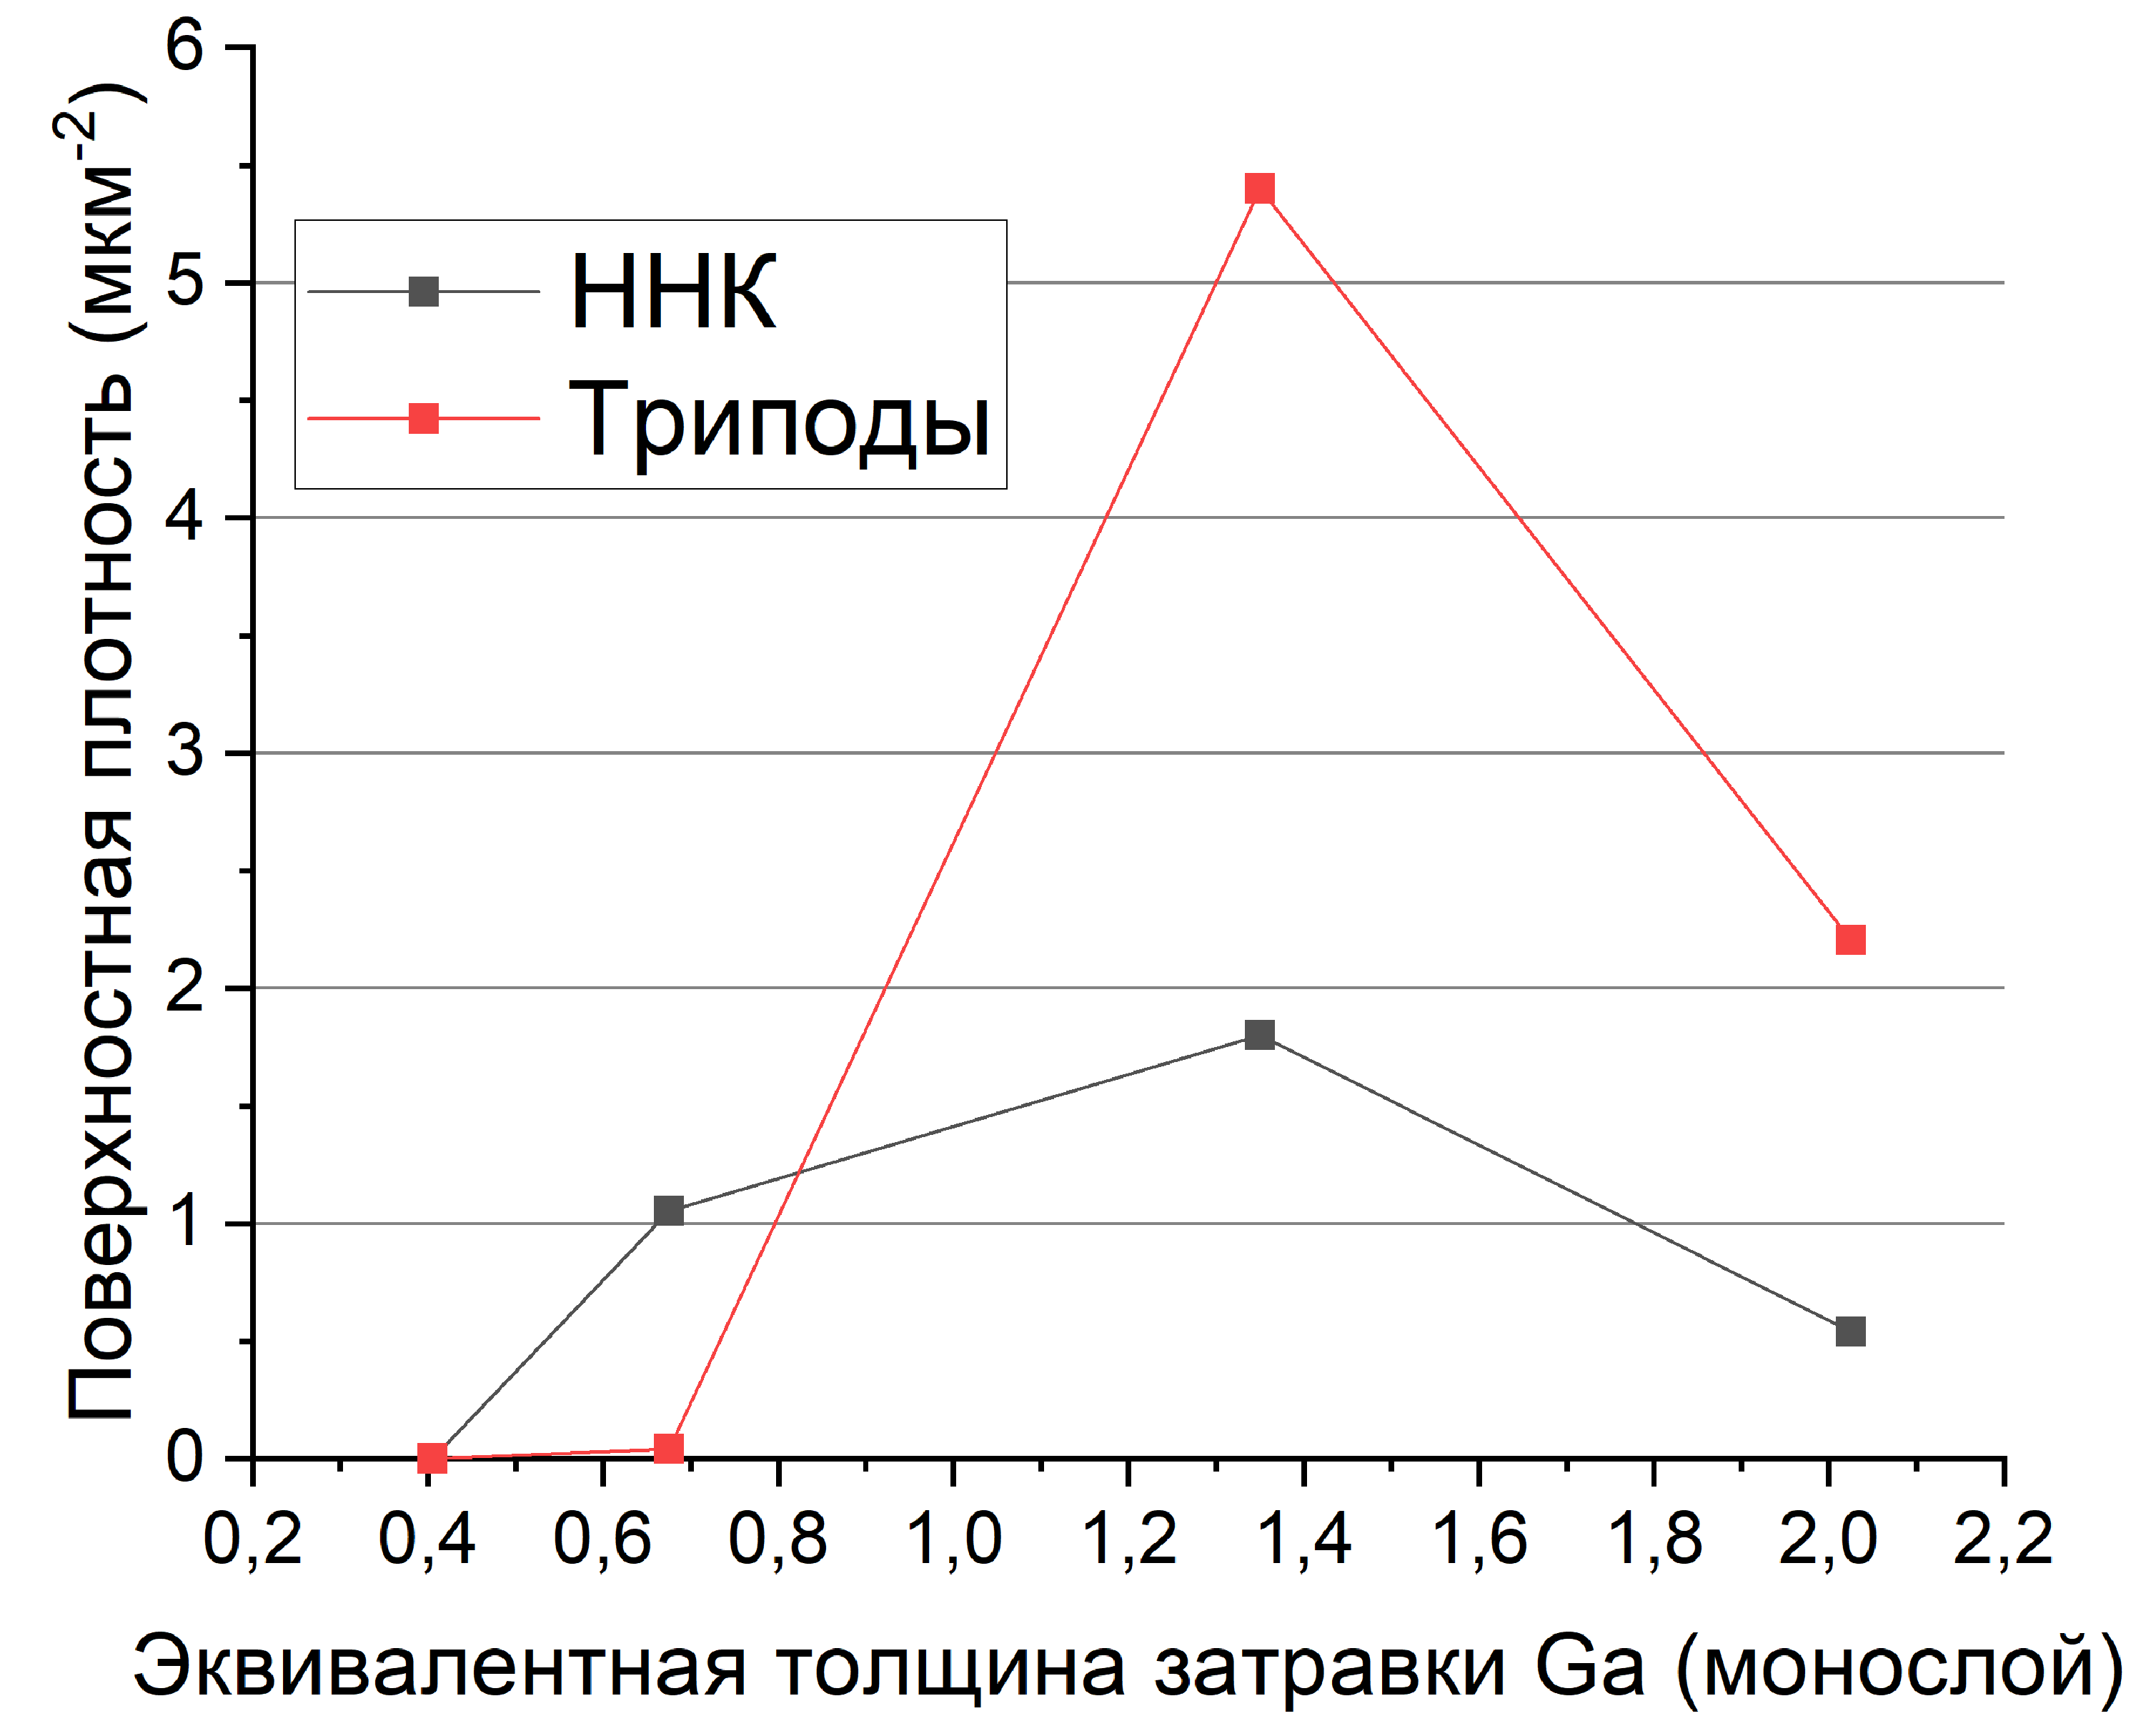
\includegraphics[width=0.48\linewidth]{Image_22_1}}
			\subcaptionbox{\label{fig:Image_22_2}}{%
		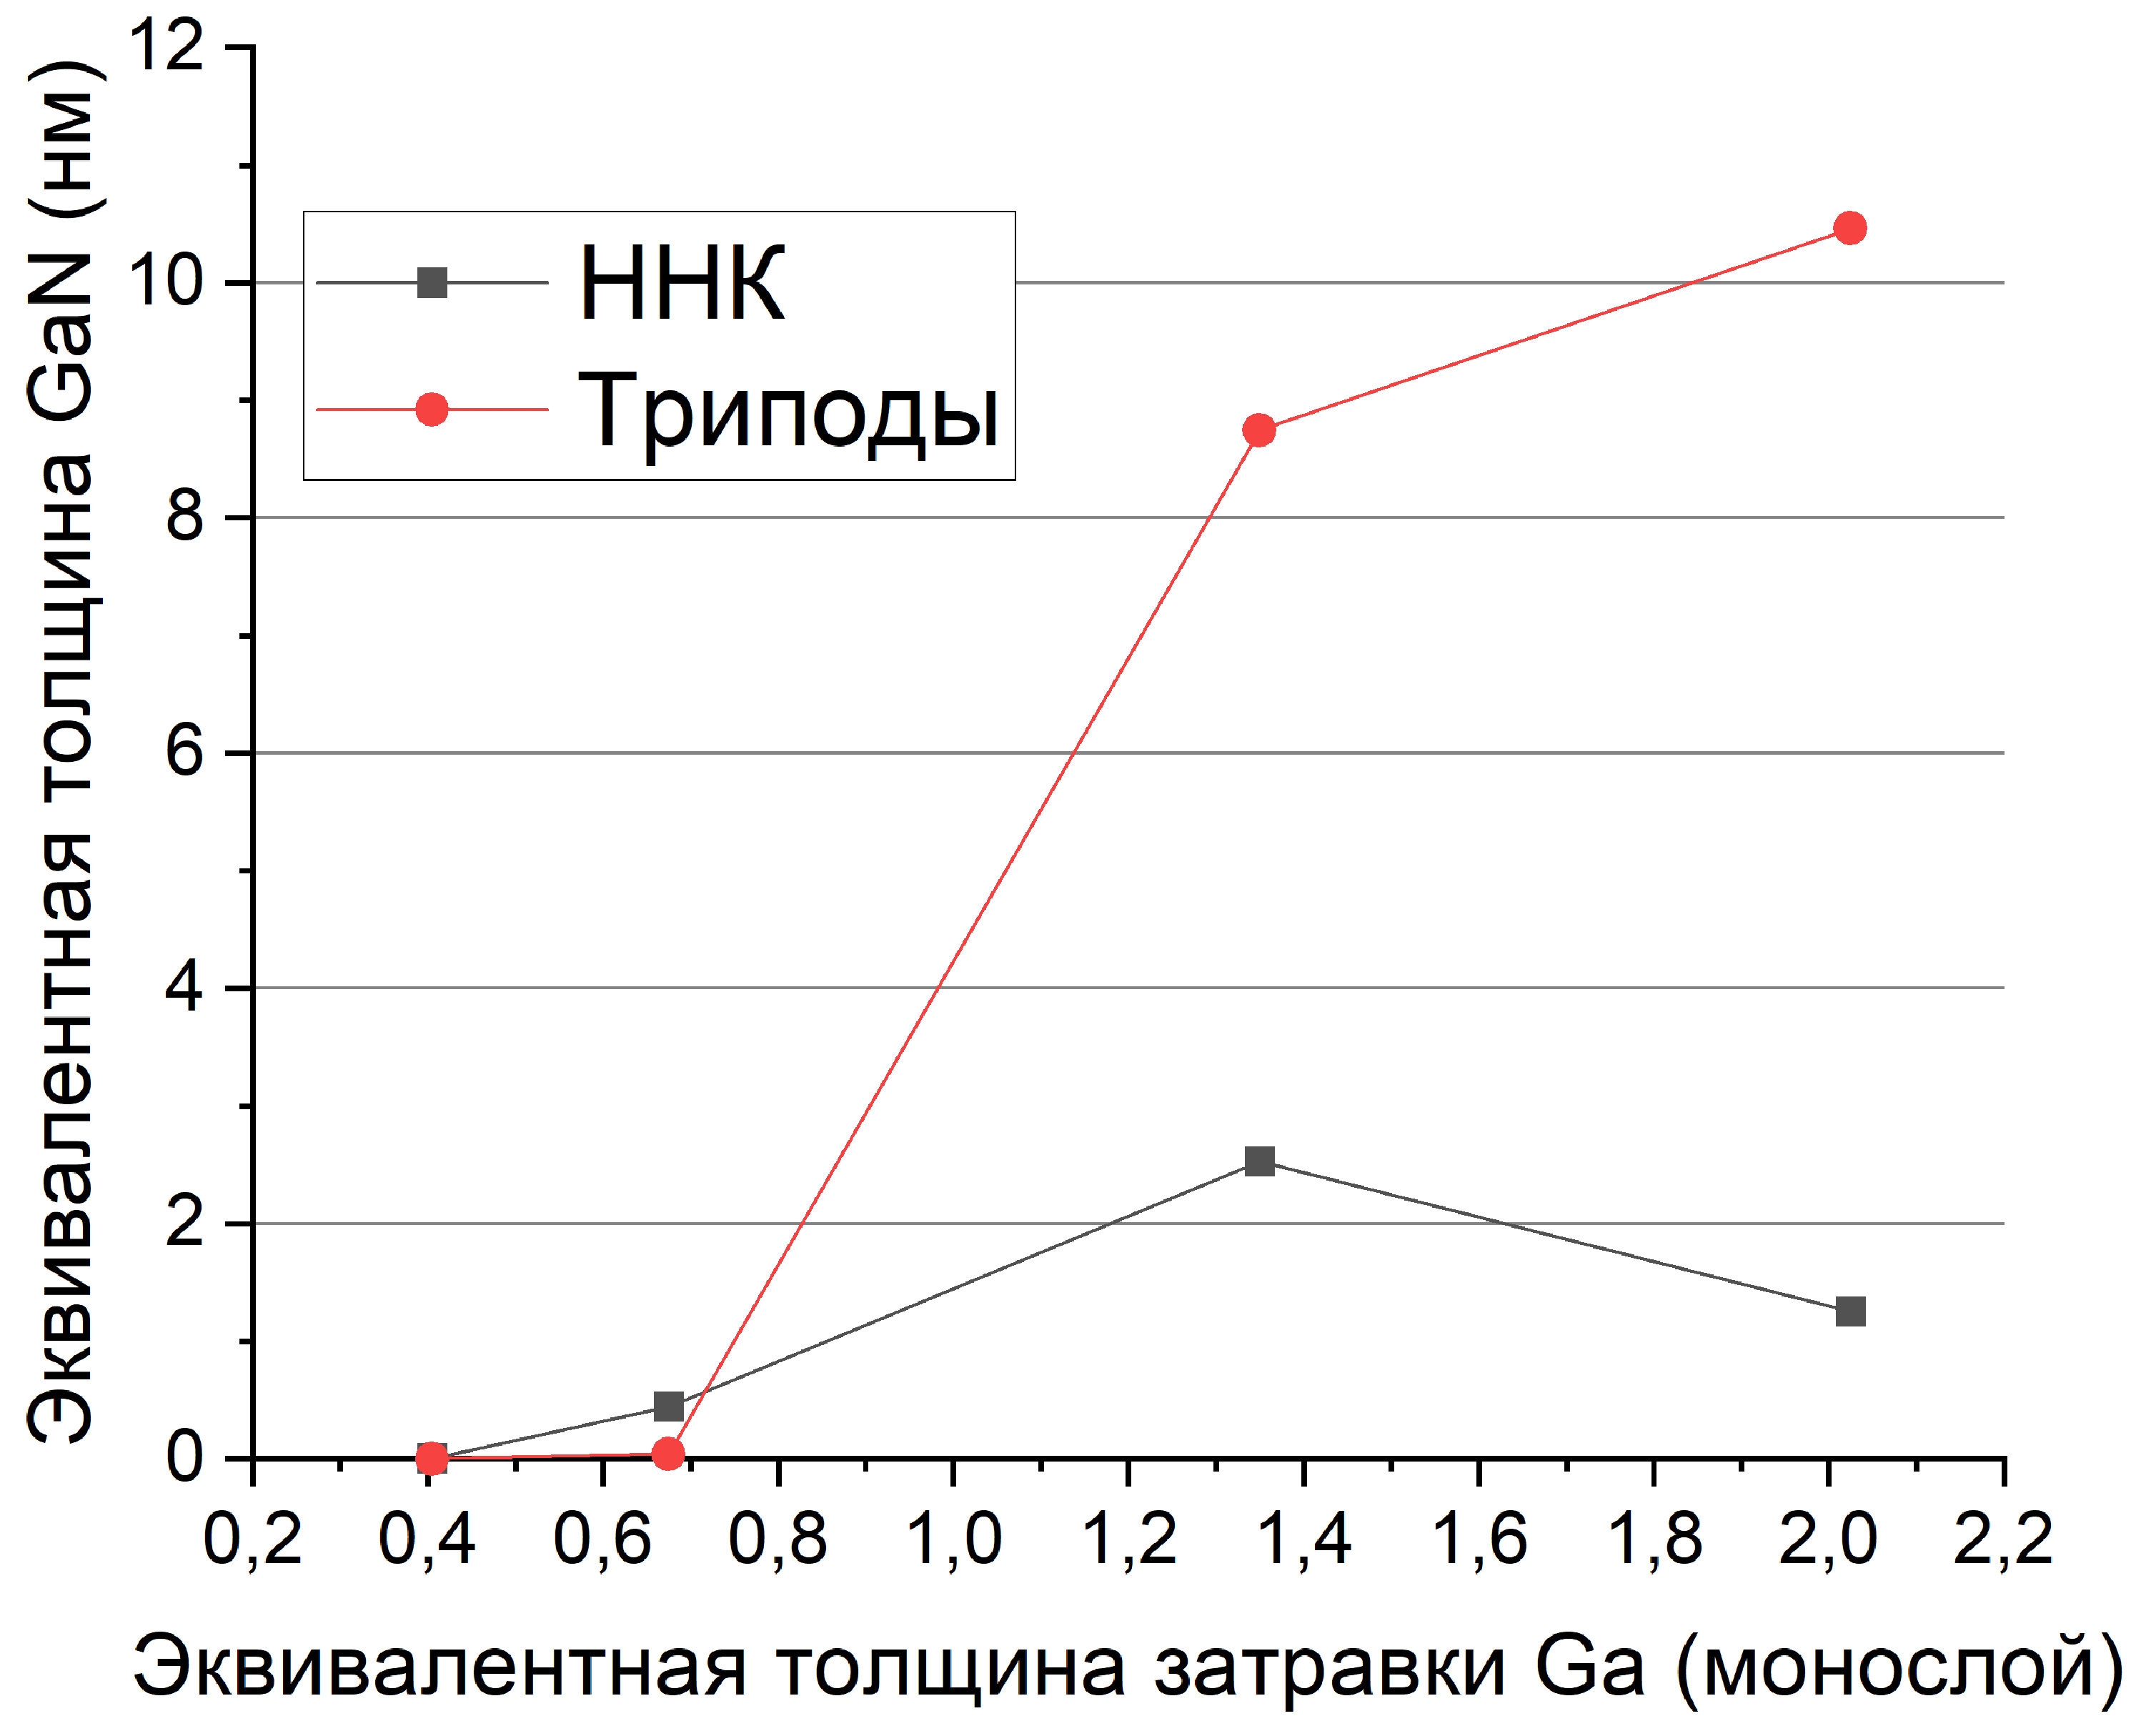
\includegraphics[width=0.48\linewidth]{Image_22_2}} } \caption{Зависимости
	эквивалентной толщины~(а) синтезированного материала и поверхностной
плотности~(б) массива наноструктур GaN от эквивалентной толщины затравочных
островков}\label{fig:Image_22} \end{figure}

Эквивалентная толщина синтезированного массива насыщается с дальнейшим
увеличением эквивалентной толщины затравочных капель. Высокая поверхностная
плотность затравочных наноостровков, служащих центрами зародышеобразования,
приводит к слиянию наноструктур массива при дальнейшем росте. Это объясняет
внезапное падение поверхностных плотностей массивов при толщине затравочного
слоя более 1,7~монослоя (см.~рис.~\cref{fig:Image_22}). Использование
затравочных капель с эквивалентной толщиной более 2,4~монослоя приводит к
формированию двумерного слоя GaN из сросшихся островков.

\subsection{Влияние соотношения молекулярных потоков
V/III}\label{subsec:ch3/sec6/sub2}

Для изучения влияния соотношения V/III на формирование триподов проведена
ростовая серия с образцами, синтезированными при различных ЭДП Ga
(см.~рис.~\cref{fig:Image_23}).

\begin{figure}[ht] \centerfloat{ \subcaptionbox{\label{fig:Image_23_1}}{%
			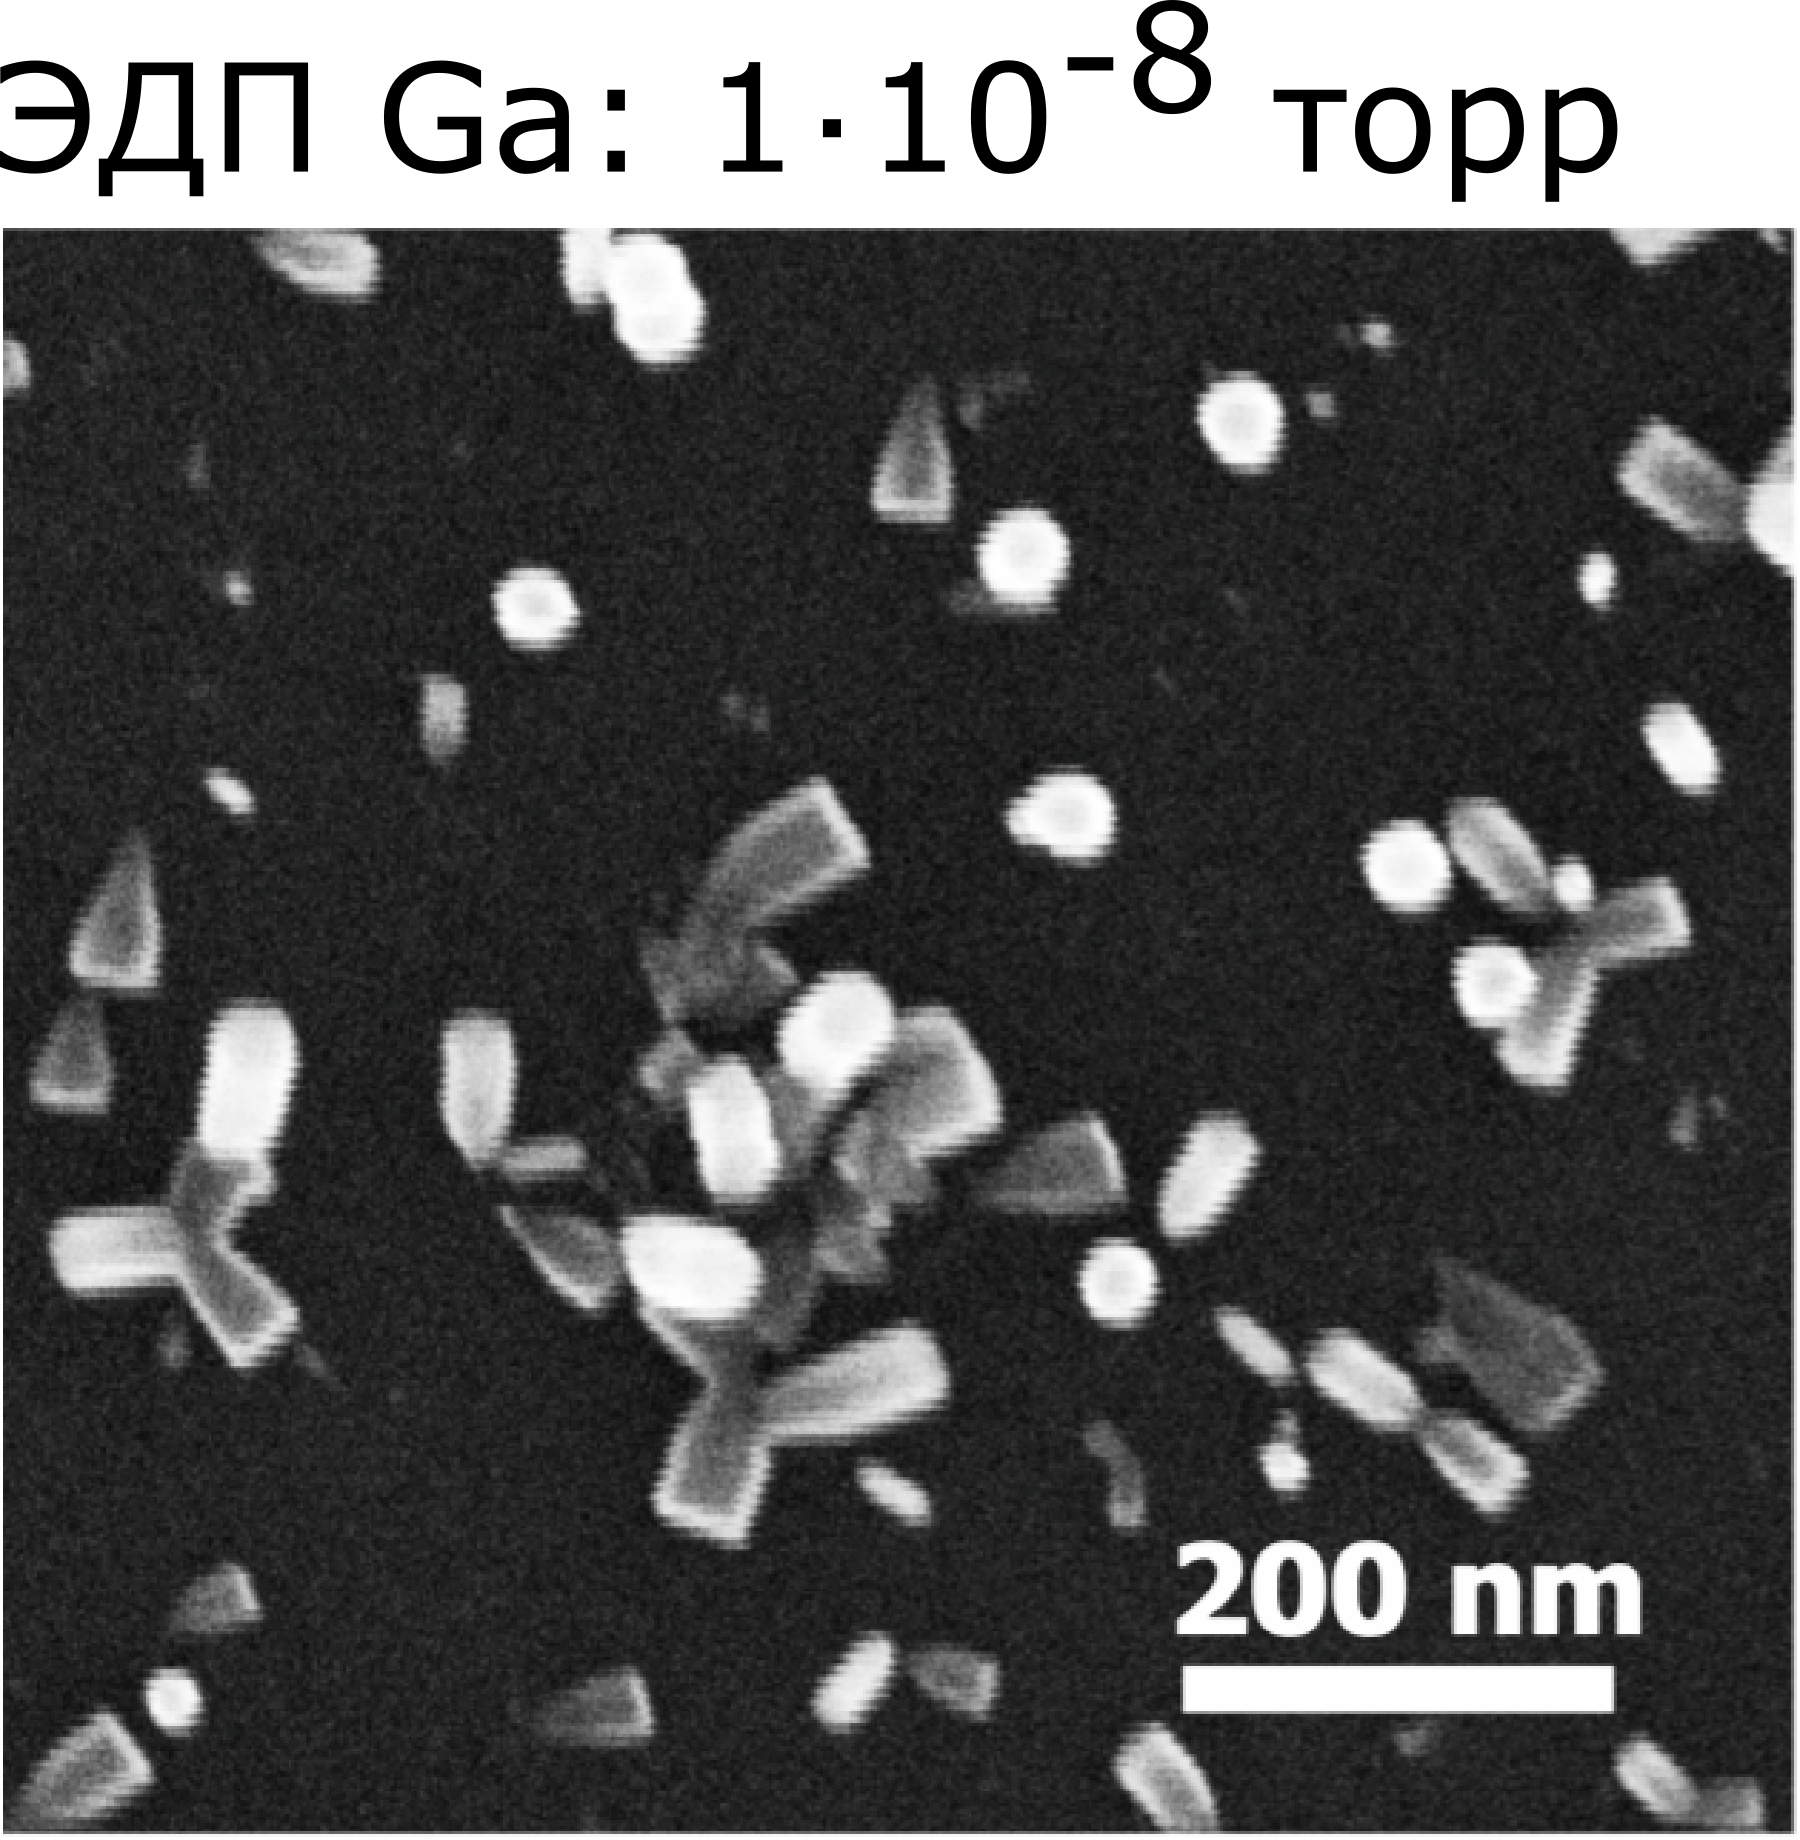
\includegraphics[width=0.25\linewidth]{Image_23_1}}
			\subcaptionbox{\label{fig:Image_23_2}}{%
				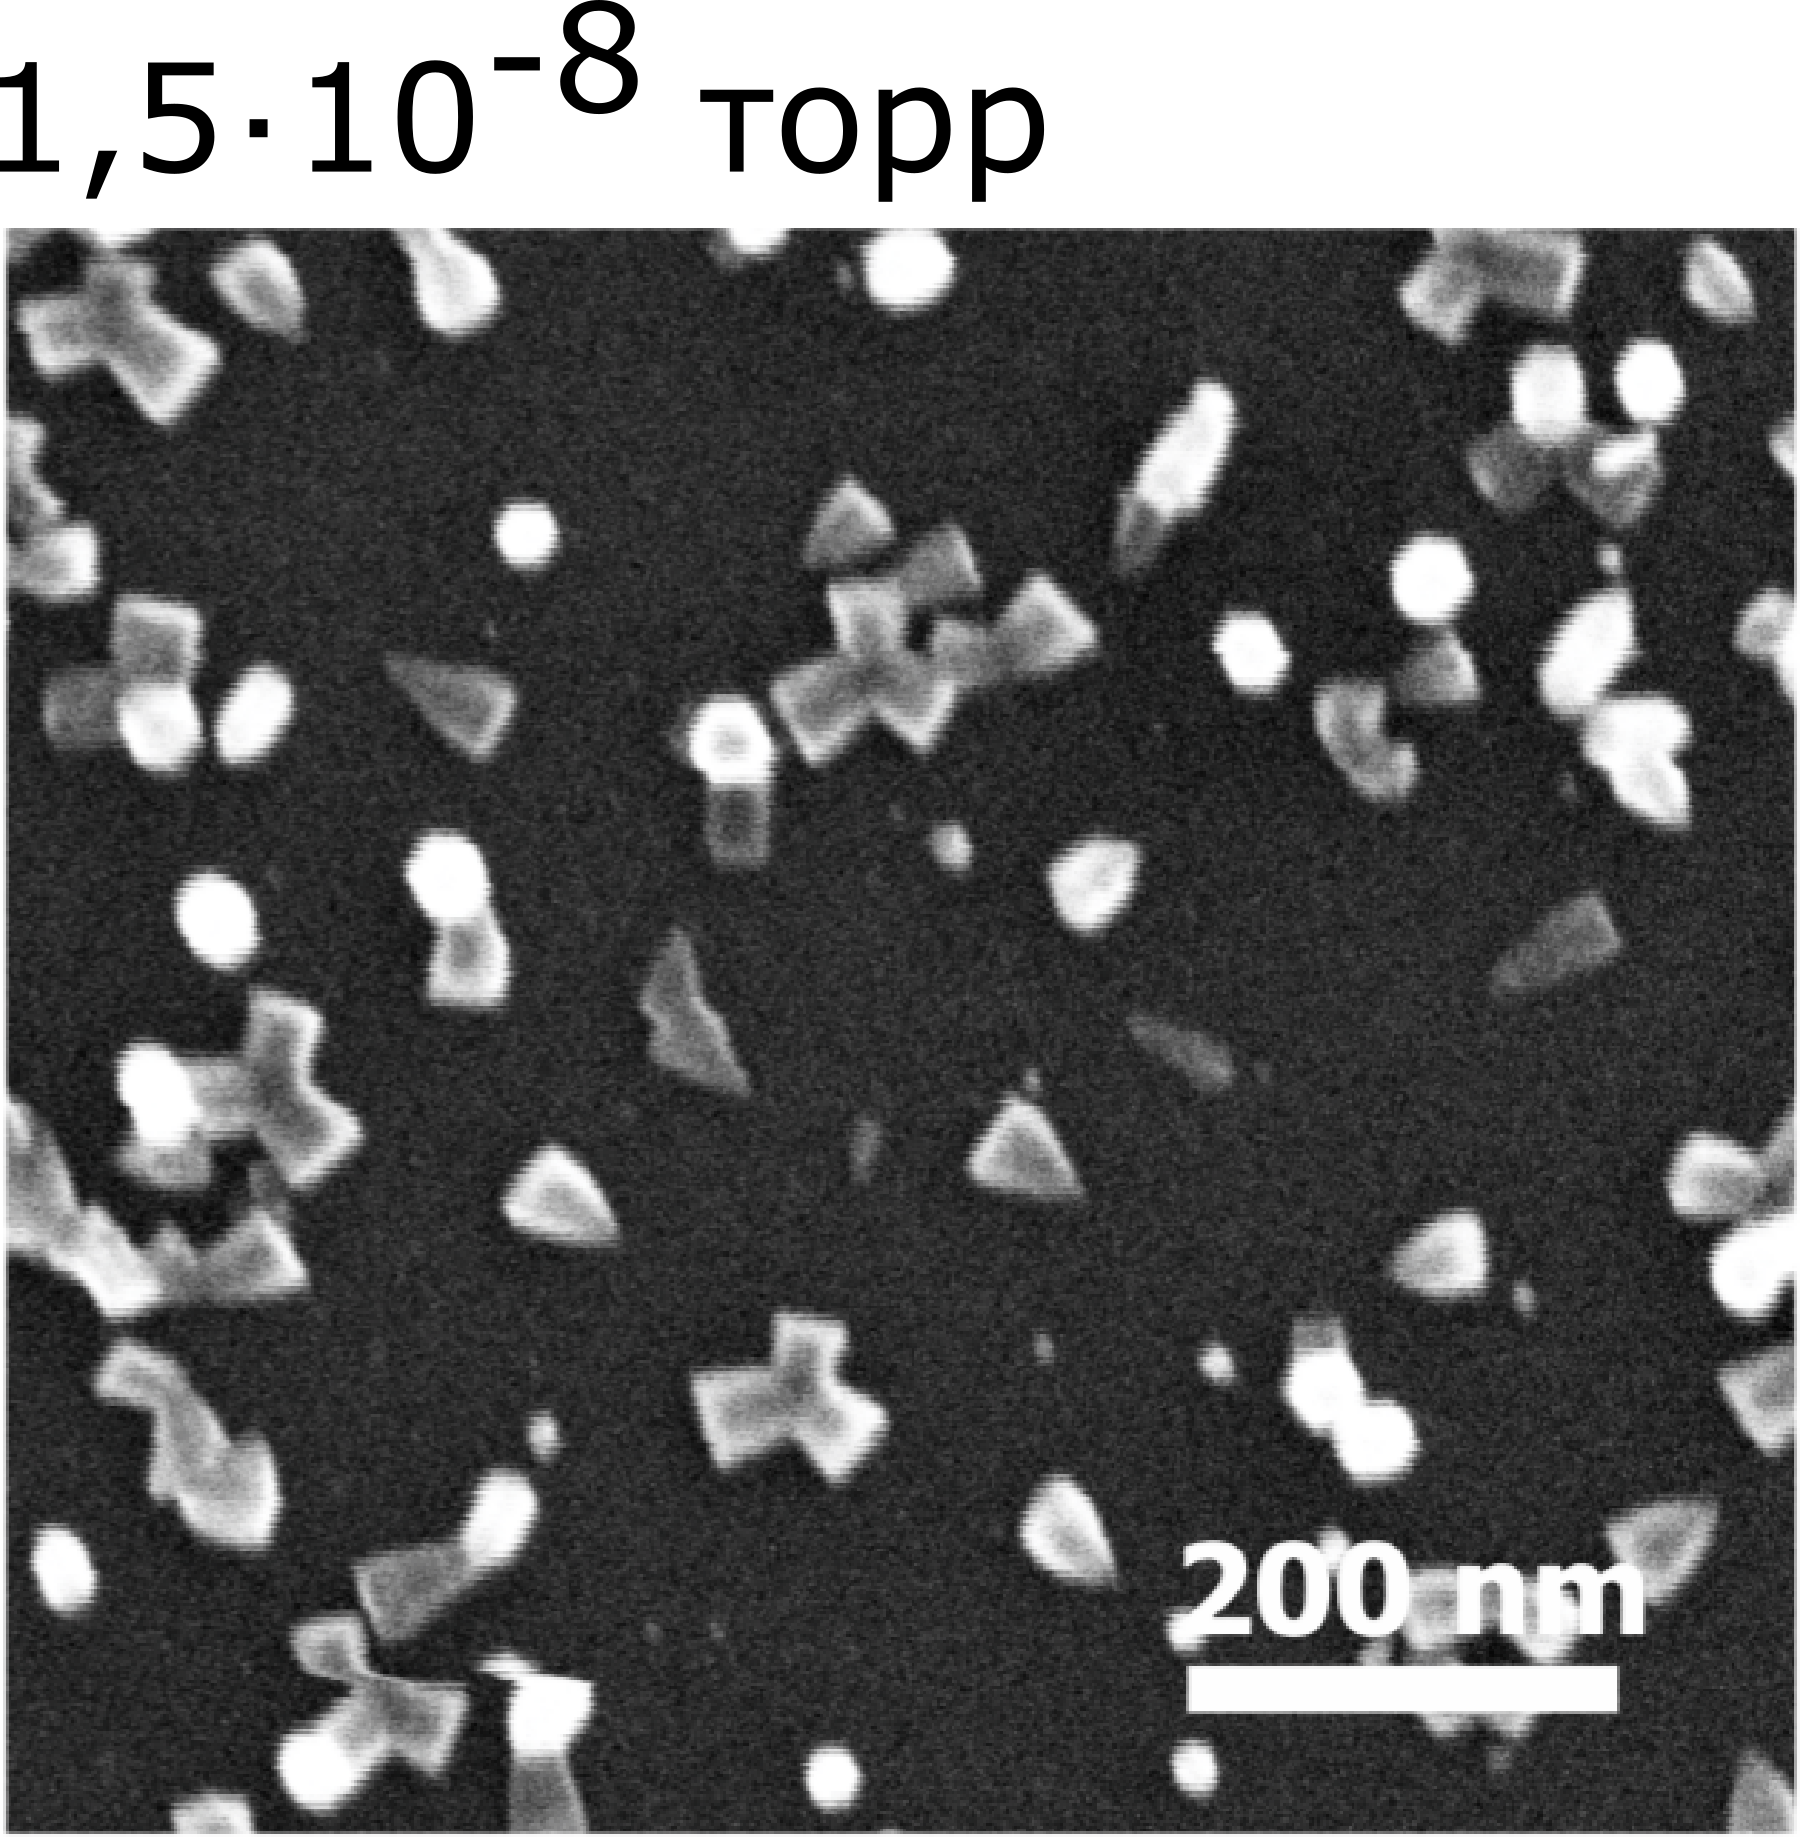
\includegraphics[width=0.25\linewidth]{Image_23_2}}
				\subcaptionbox{\label{fig:Image_23_3}}{%
			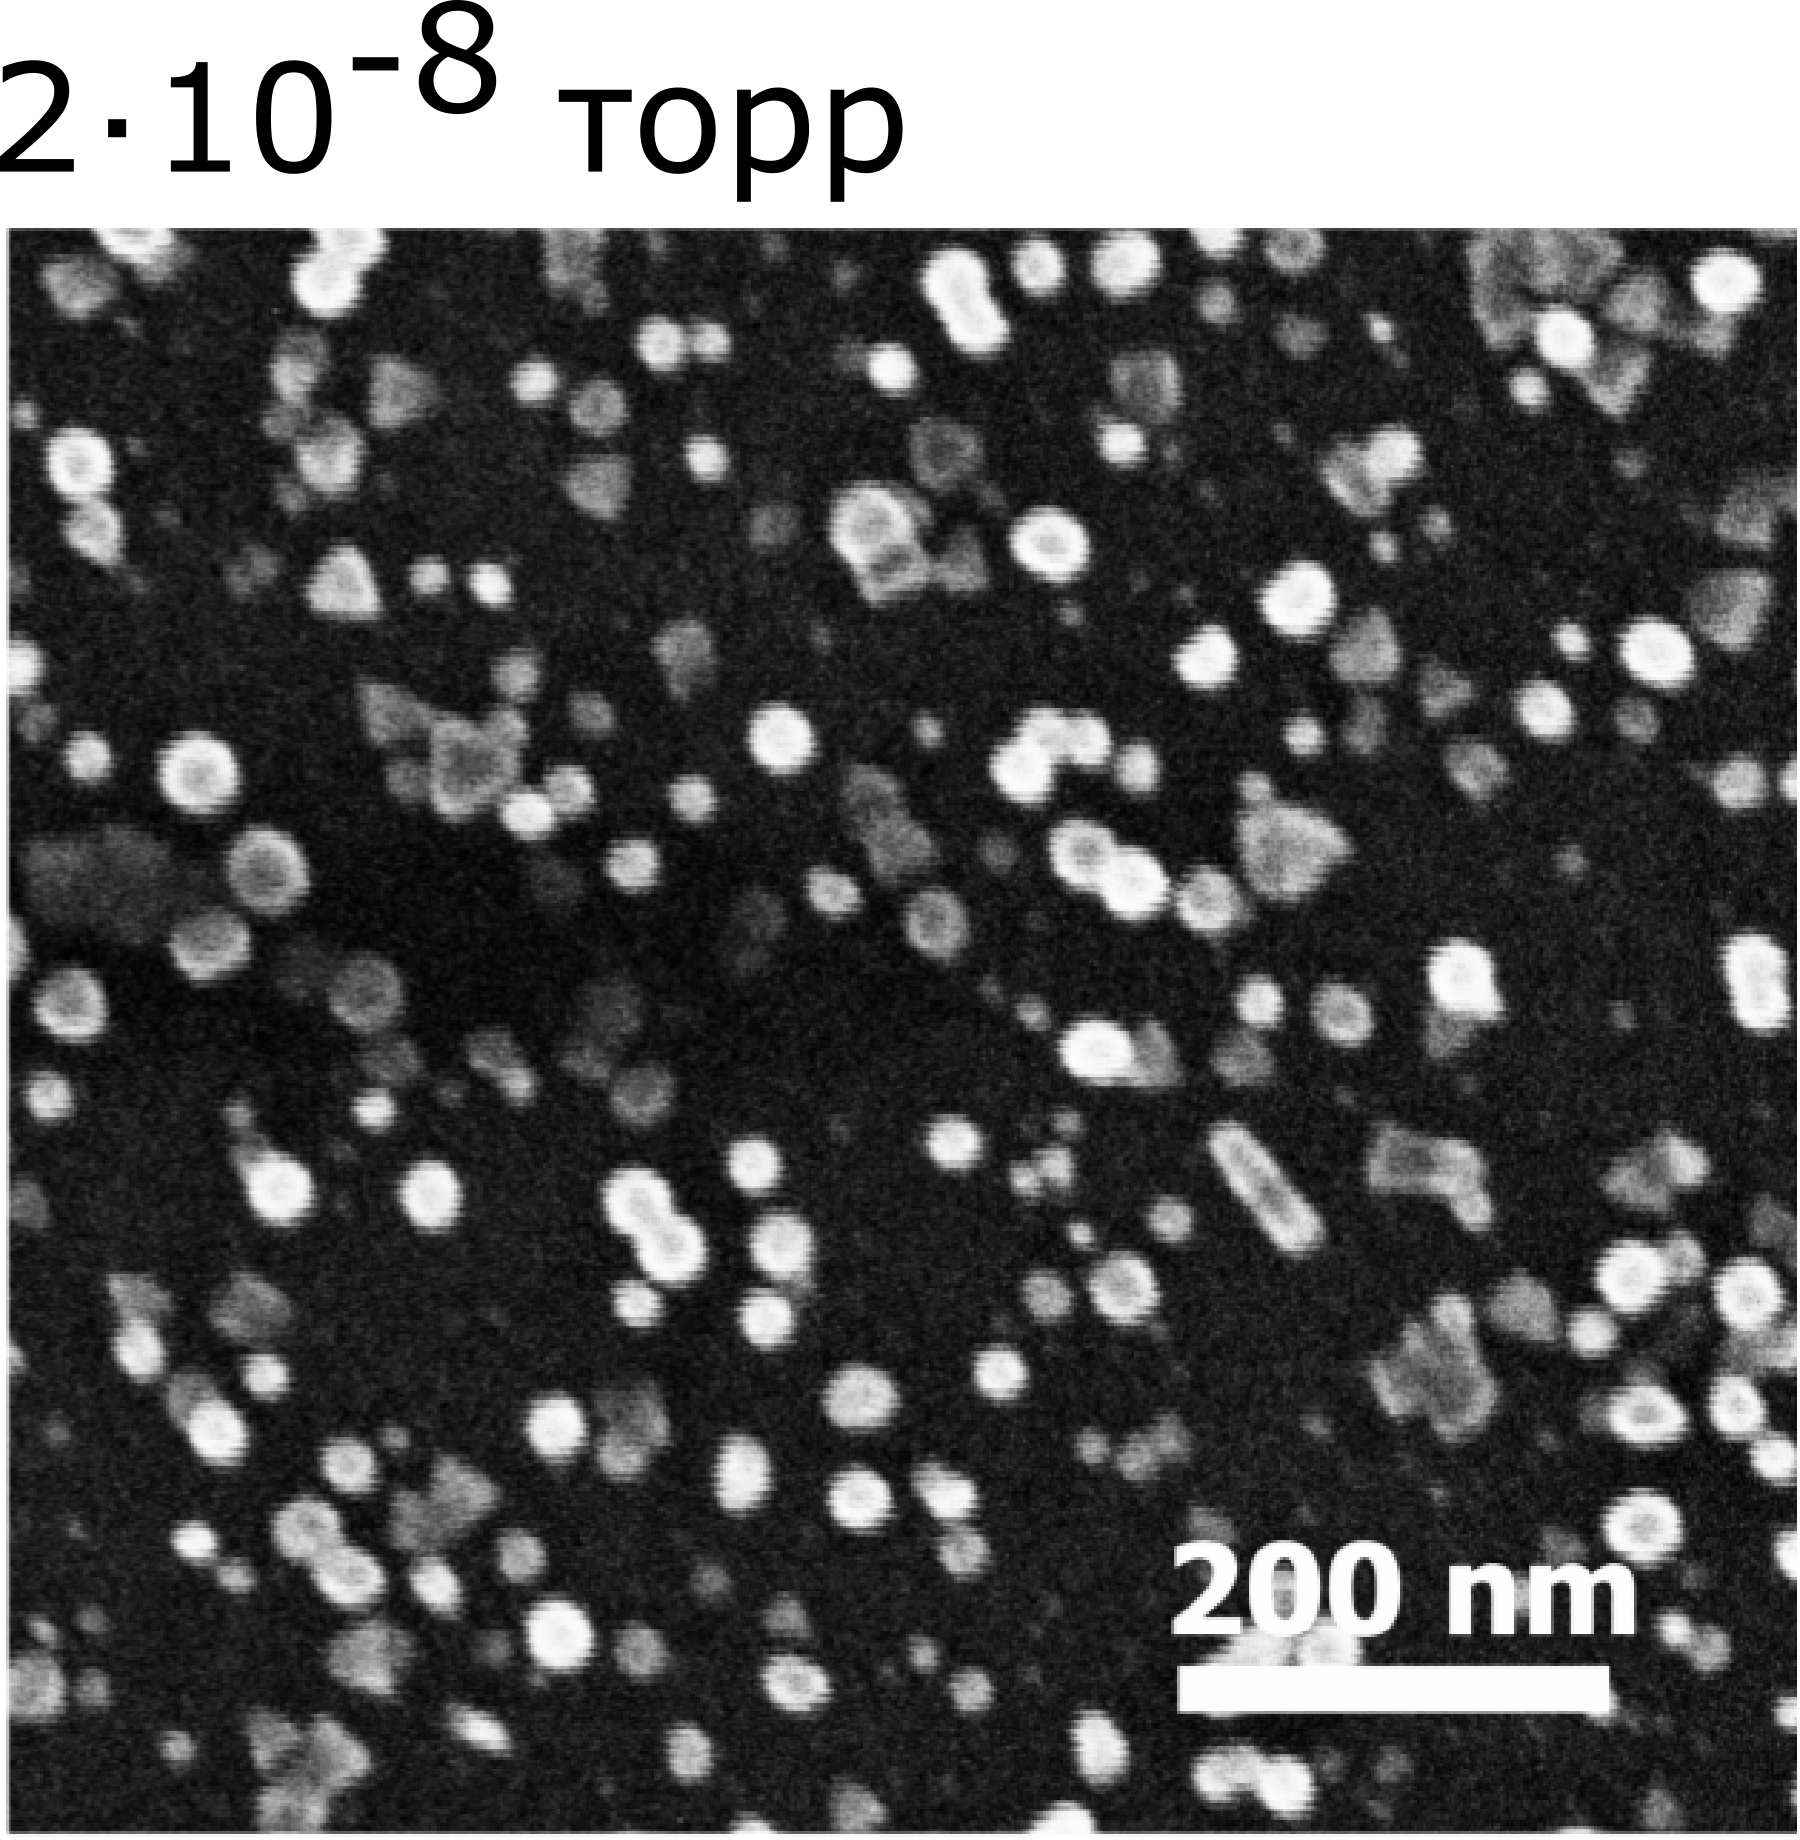
\includegraphics[width=0.25\linewidth]{Image_23_3}} } \legend{ЭДП Ga \(1
		\cdot 10^{-8}\)~(а), \(1,5 \cdot 10^{-8}\)~(б), \(2 \cdot
	10^{-8}\)~\si{\torr}~(в)} \caption{РЭМ изображения наноструктур GaN,
выращенных при различных ЭДП Ga}\label{fig:Image_23} \end{figure}

Согласно работе \cite{Voulot1998}, расход азота или ВЧ мощность влияет не
только на ЭДП активированного азота, но и на соотношение в нем атомов, молекул
и ионов \cite{Blant2000}, поэтому корреляции между расходом азота и потоком
активированного азота нелинейная. По этой причине параметры источника плазмы
сохранялись постоянными (расход азота 1~\si{\centi\meter^3\per\minute}, ВЧ
мощность 500~\si{\watt}).

Увеличение ЭДП Ga в исследуемом диапазоне уменьшает скорость роста вертикальных
и наклоненных ННК, снижает аспектное отношение ННК и триподов (длина/толщина)
(см.~рис.~\cref{fig:Image_24_1},~ \cref{fig:Image_24_2}), повышает сужение ННК
у основания. Поверхность подложки в основном занята триподами при ЭДП Ga \(1,5
\cdot 10^{-8}\)~\si{\torr}, а при потоке выше и ниже этого значения на
поверхности доминируют ННК (см.~рис.~\cref{fig:Image_24_1}).

\begin{figure}[ht] \centerfloat{ \subcaptionbox{\label{fig:Image_24_1_1}}{%
			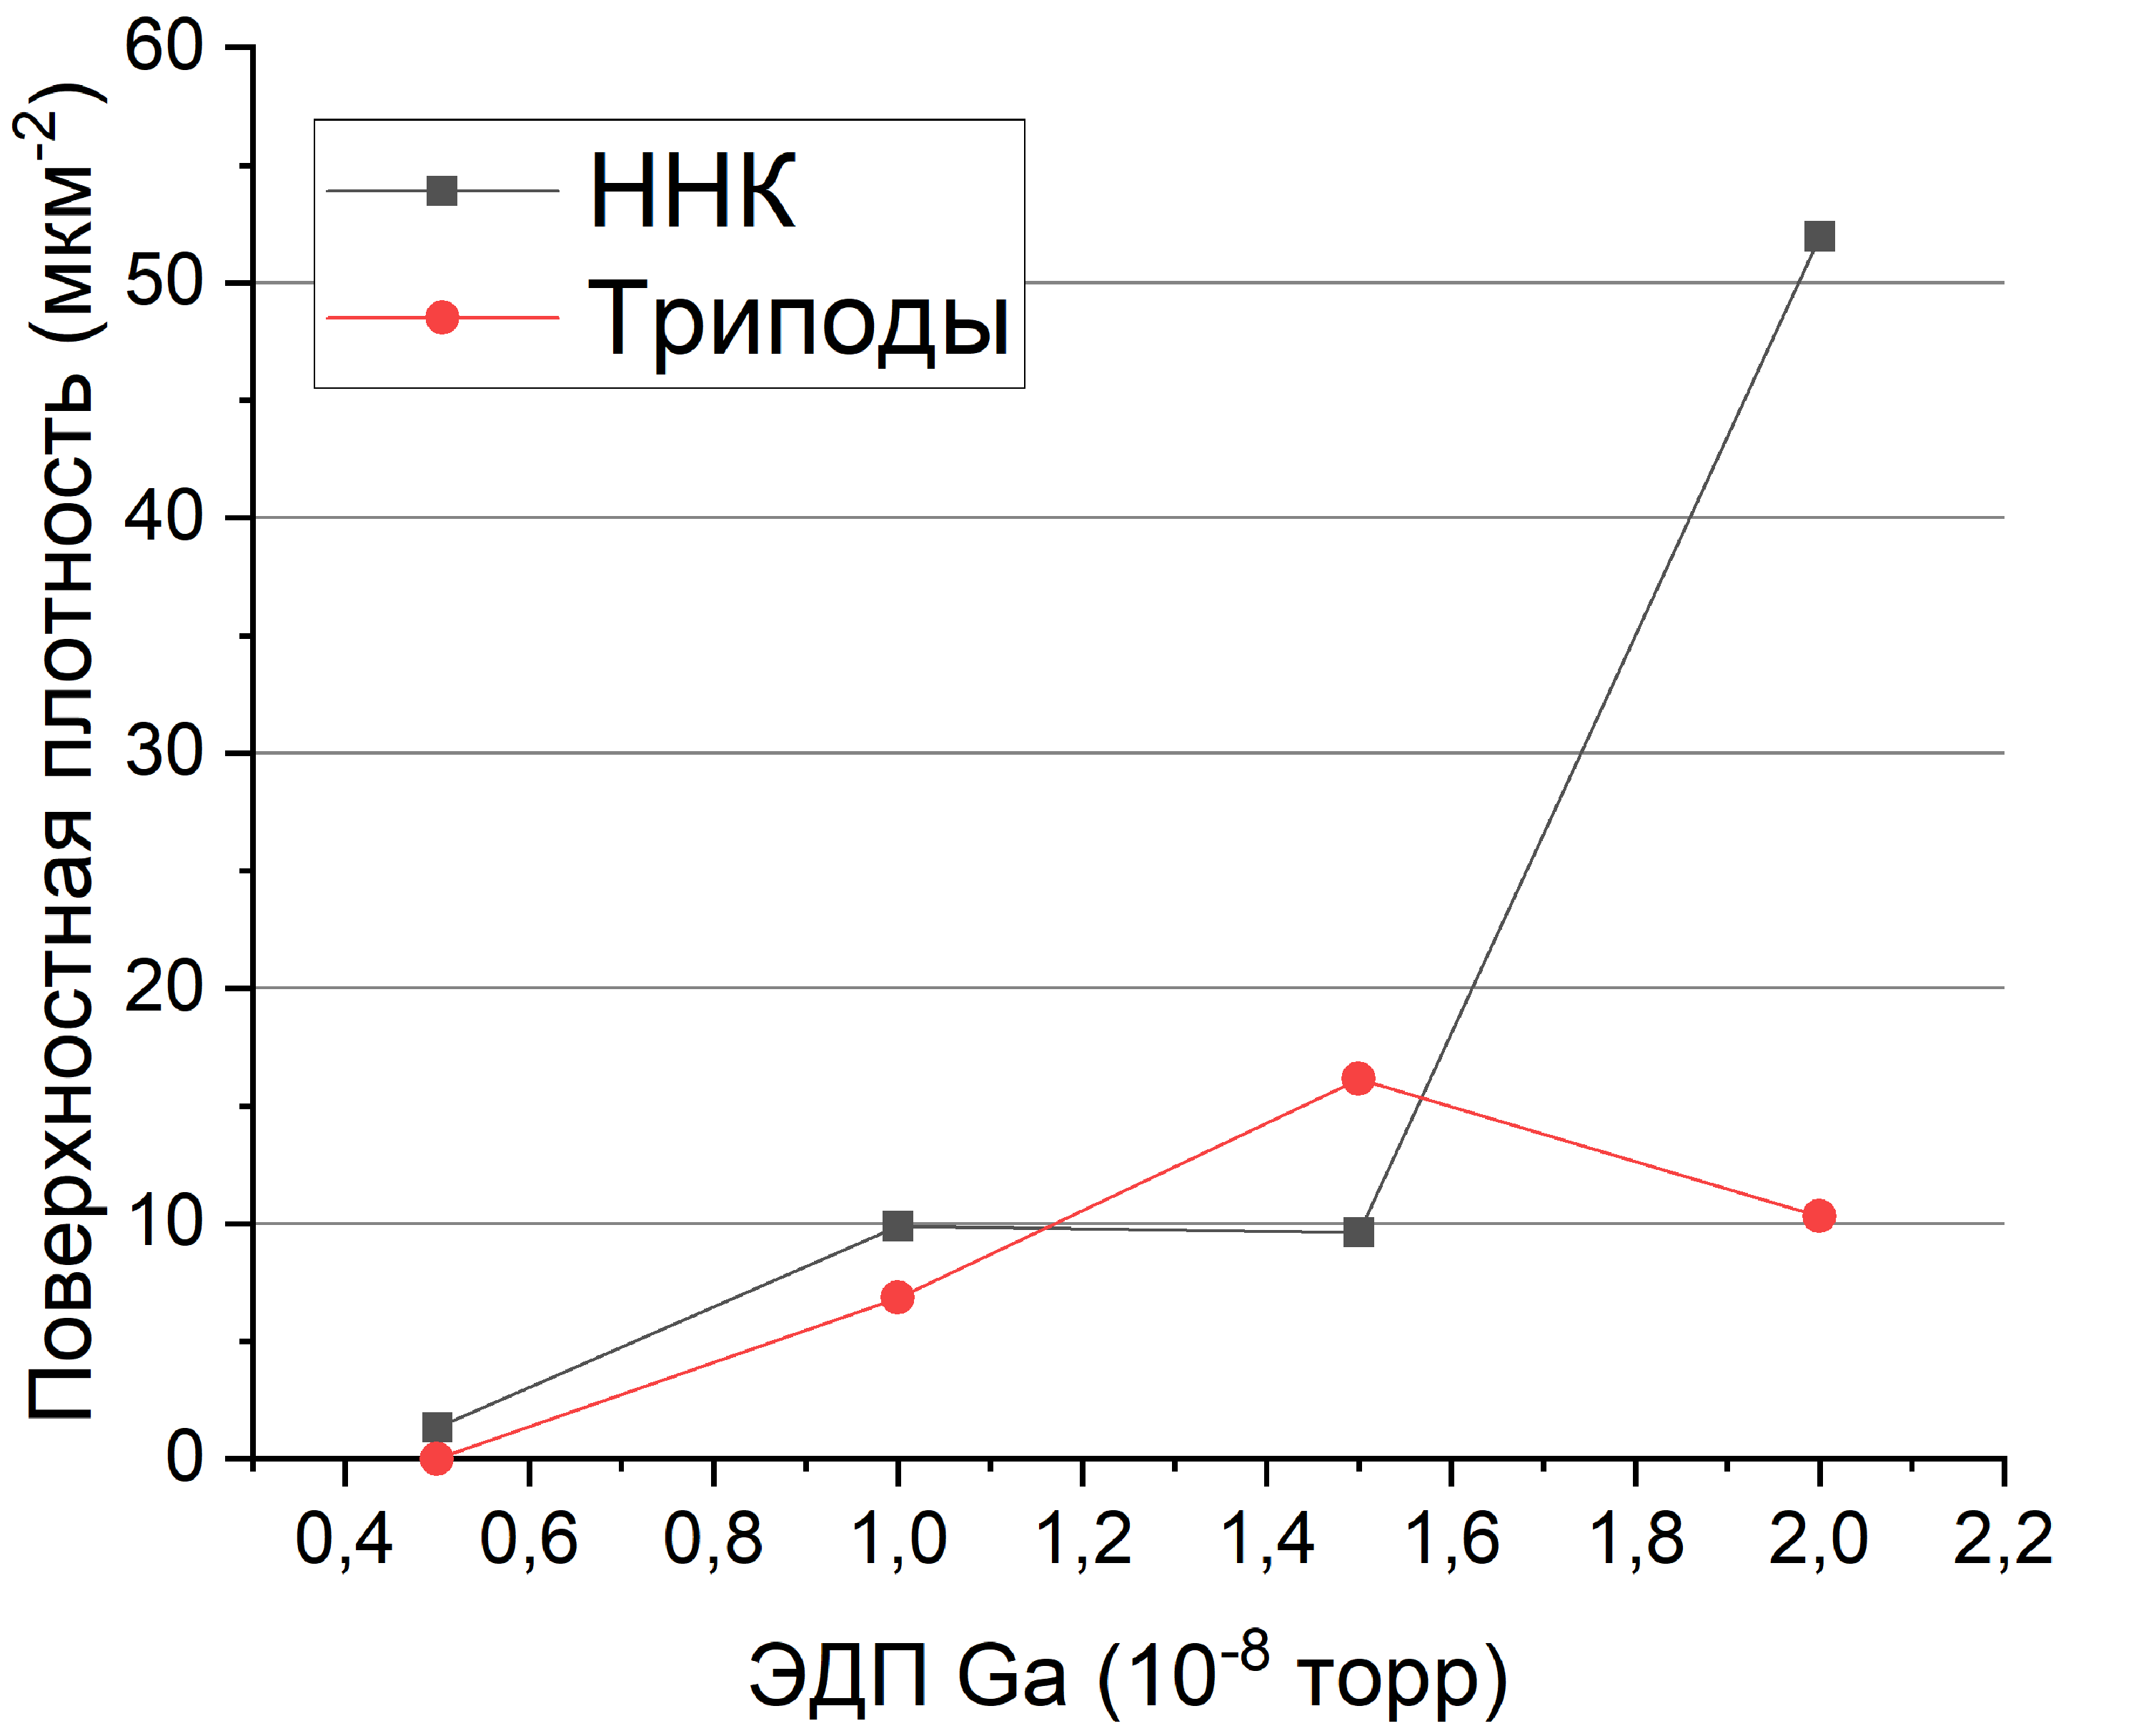
\includegraphics[width=0.48\linewidth]{Image_24_1_1}}
			\subcaptionbox{\label{fig:Image_24_1_2}}{%
		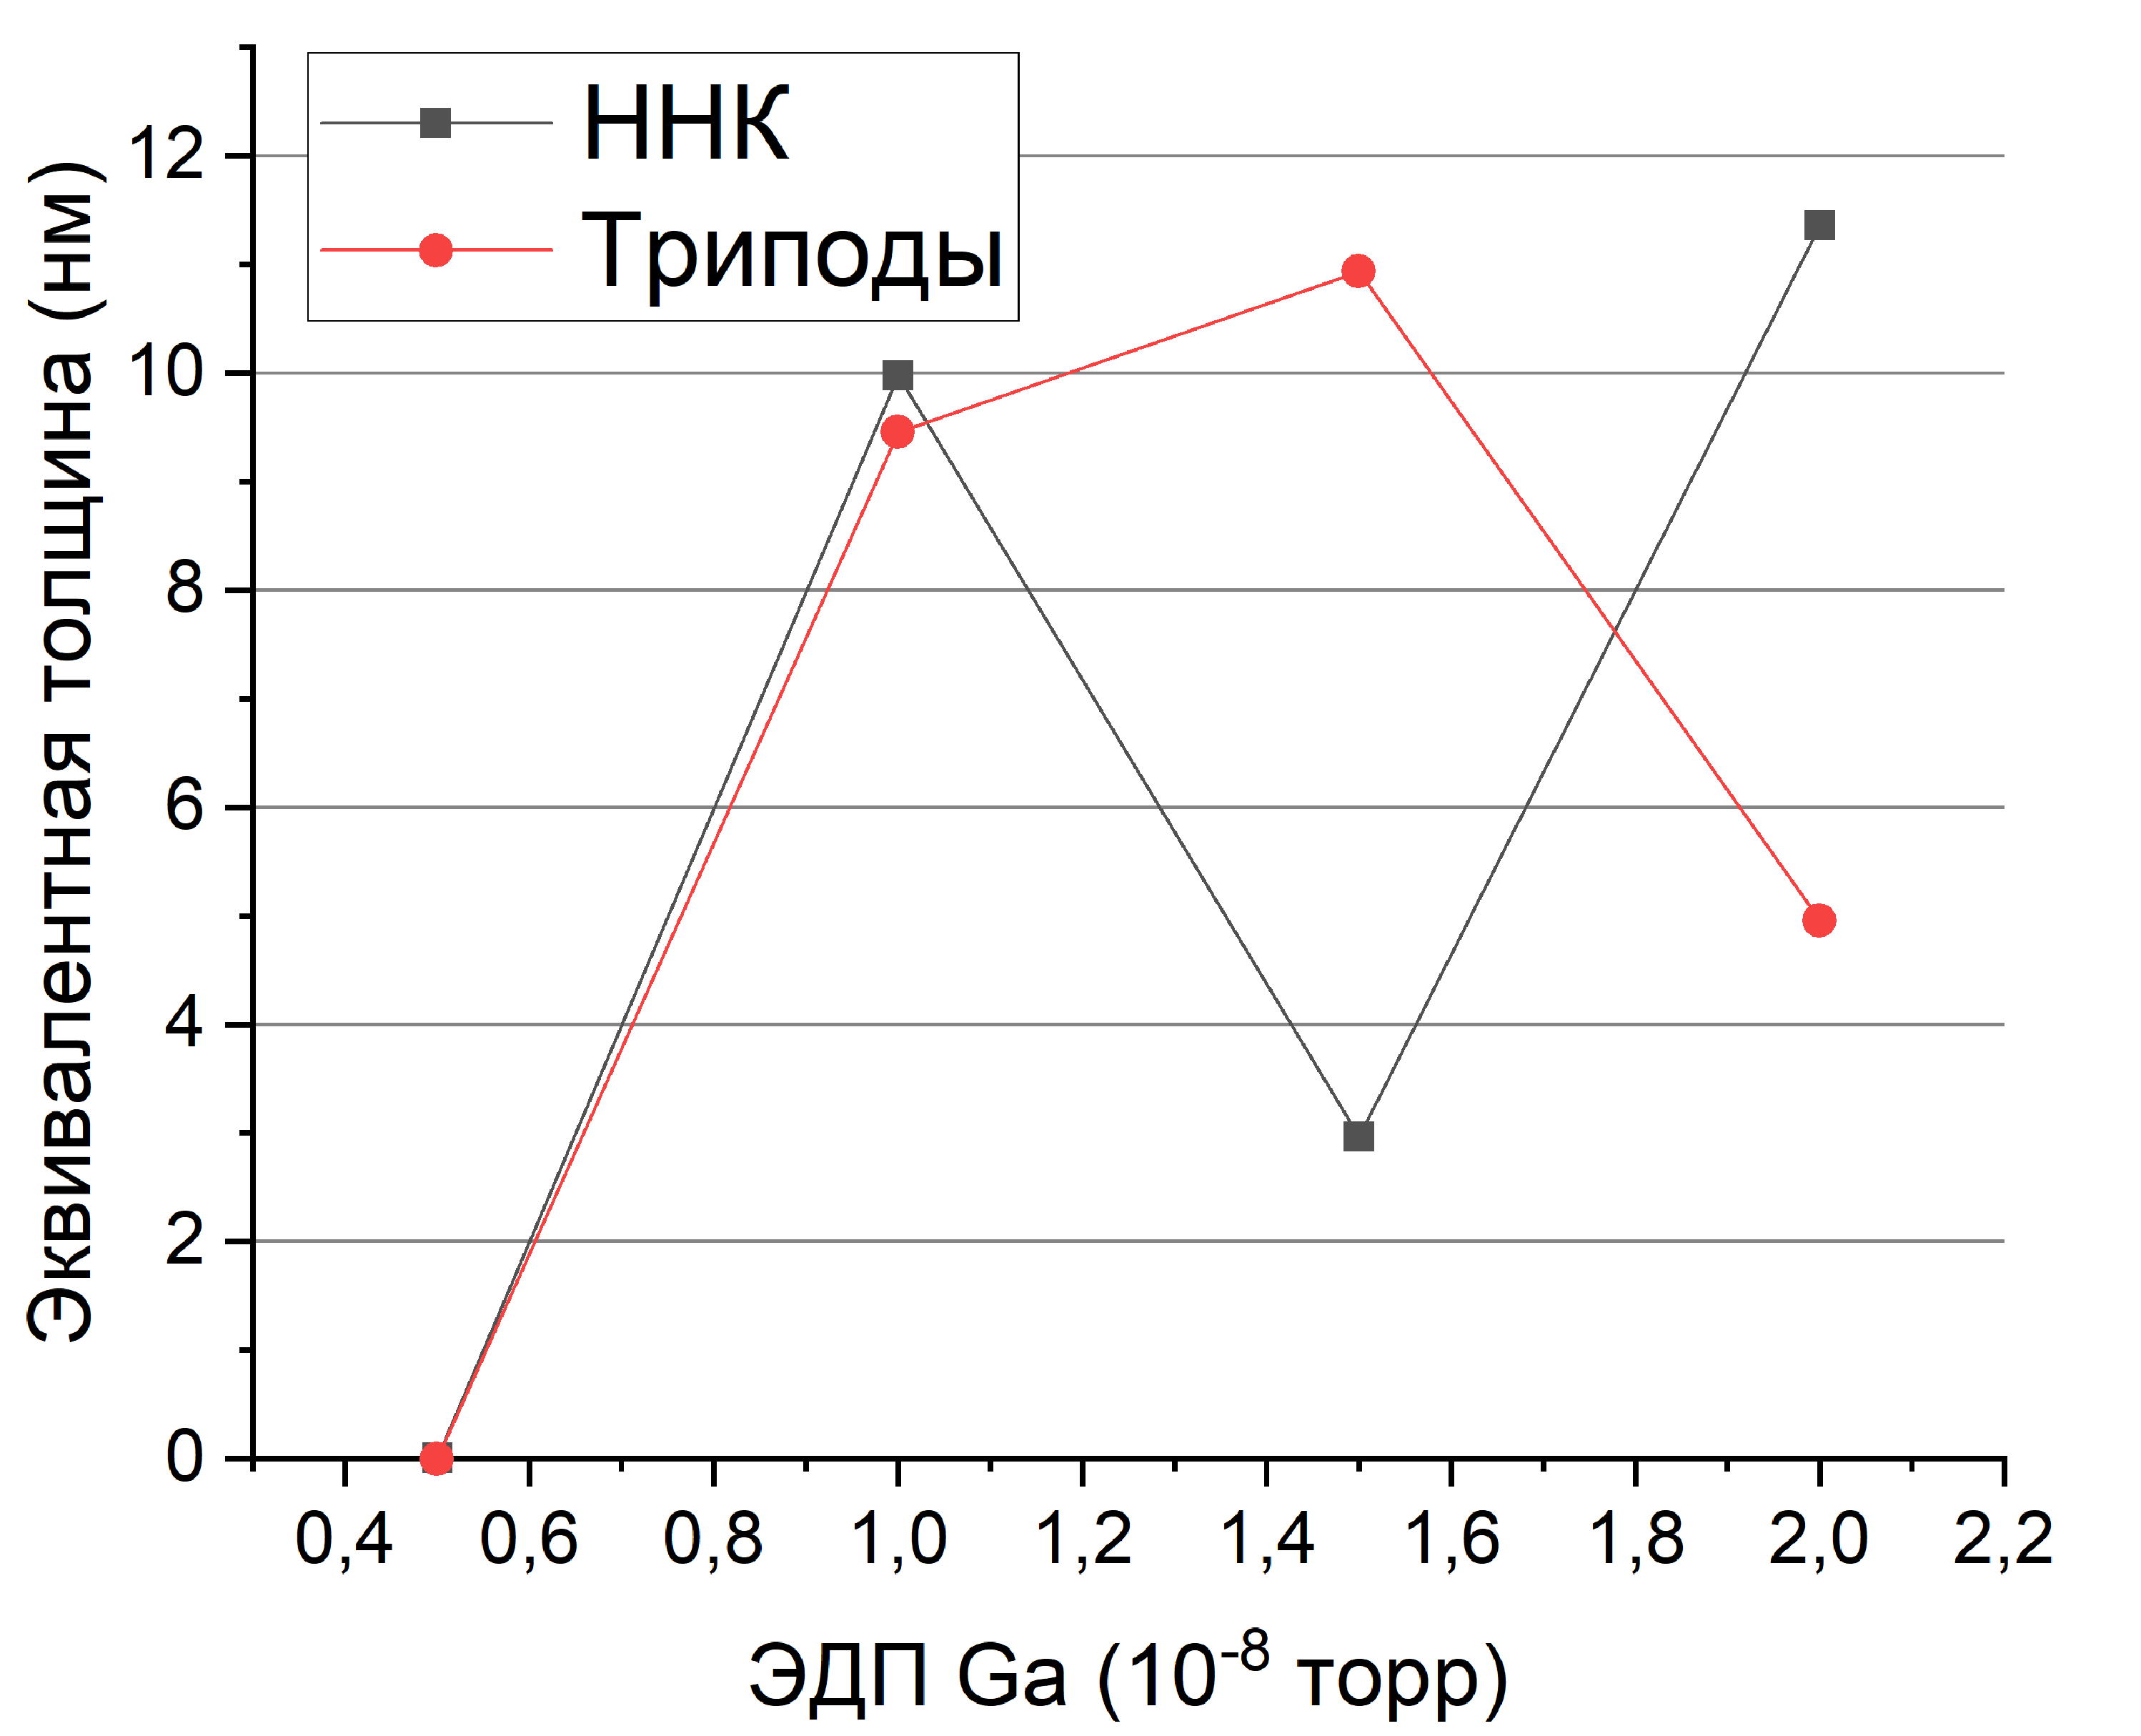
\includegraphics[width=0.48\linewidth]{Image_24_1_2}} }
		\caption{Зависимости поверхностной плотности~(а) и эквивалентной толщины
		осажденного материала~(б) наноструктур GaN от ЭДП Ga}\label{fig:Image_24_1}
	\end{figure}

\begin{figure}[ht] \centerfloat{
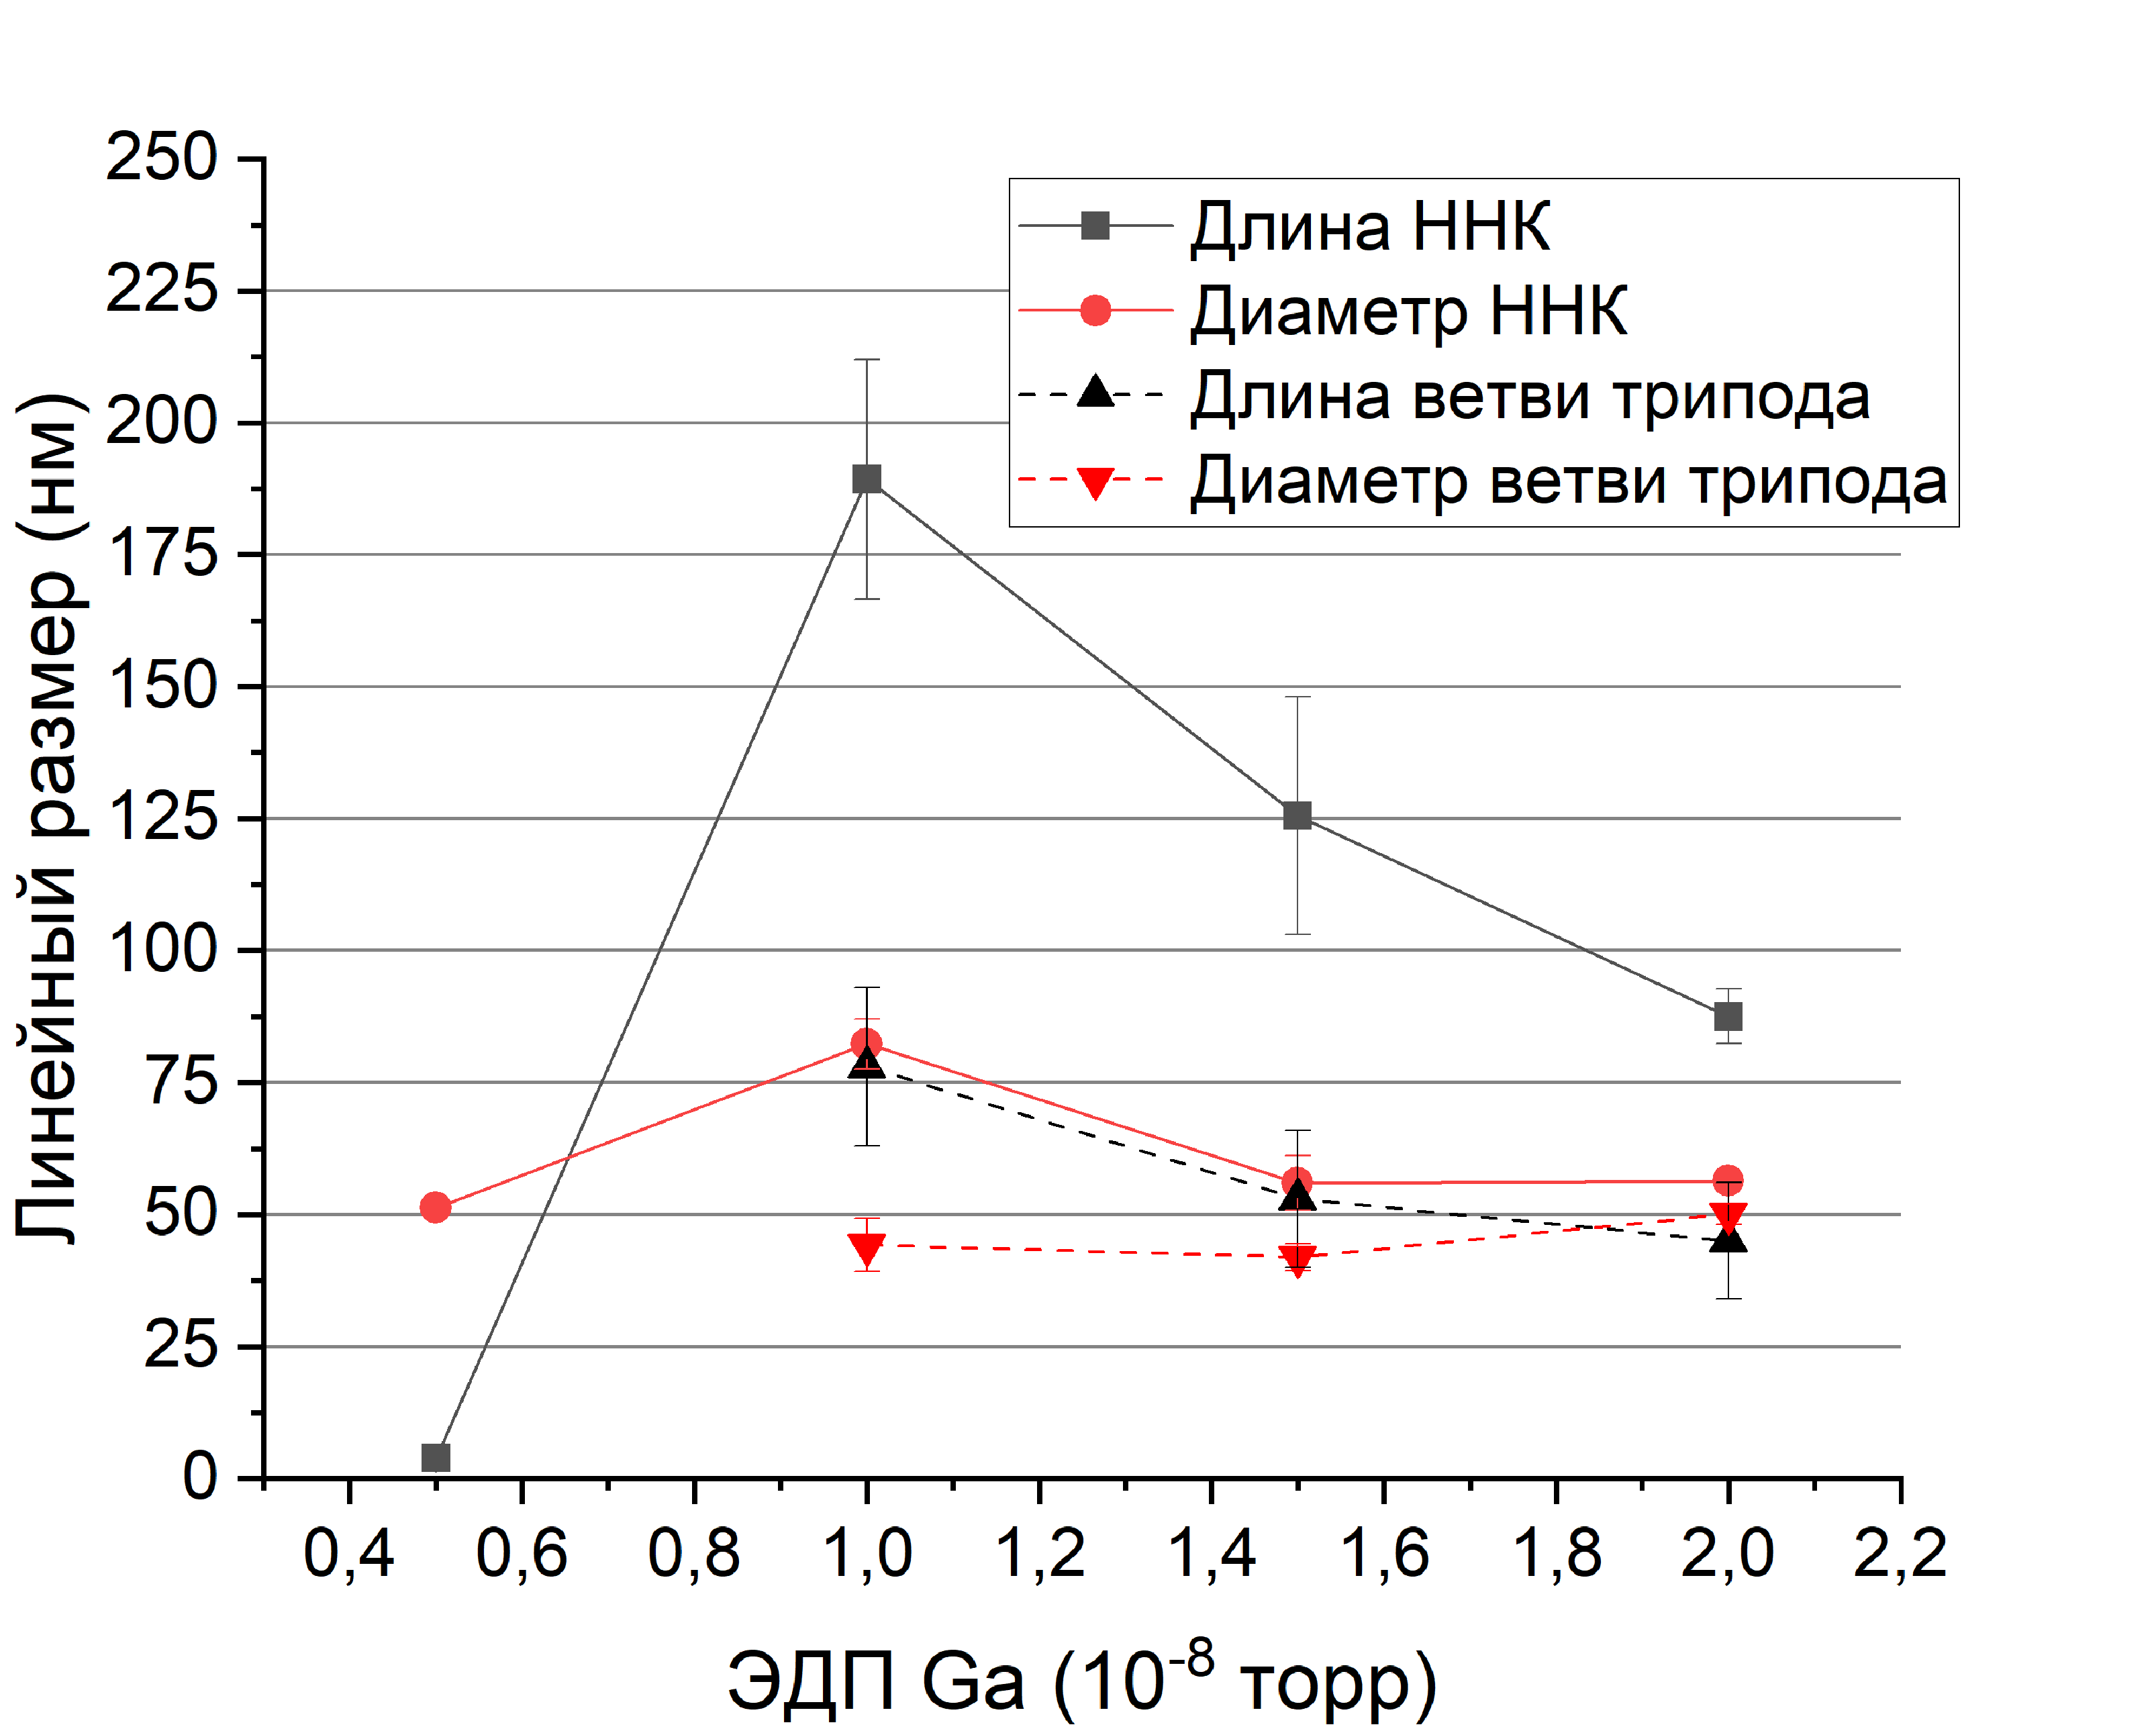
\includegraphics[width=0.6\linewidth]{Image_24_2} } \caption{Зависимости
линейных размеров наноструктур GaN от ЭДП Ga}\label{fig:Image_24_2}
\end{figure}

Эквивалентная толщина осаждаемого материала (см.~рис.~\cref{fig:Image_24_1_2})
не пропорциональна ЭДП Ga~--- увеличение поверхностной плотности
(см.~рис.~\cref{fig:Image_24_1_1}) компенсируется уменьшением среднего
поперечного размера наноструктур (см.~рис.~\cref{fig:Image_24_2}).

\subsection{Влияние ростовой температуры подложки}\label{subsec:ch3/sec6/sub3}

Наноструктуры формировались в узком температурном диапазоне с 690 до
710~\si{\degreeCelsius} (см.~рис.~\cref{fig:Image_25}). При температуре роста
690~\si{\degreeCelsius} поверхностная плотность триподов становится настолько
высокой, что они срастаются и покрывают почти всю поверхность подложки
(см.~рис.~\cref{fig:Image_26_1_1}). Поверхностная плотность наноструктур быстро
падает с температурой. Формирование триподов полностью подавляется при
температурах выше 705~\si{\degreeCelsius}.

\begin{figure}[ht] \centerfloat{ \subcaptionbox{\label{fig:Image_25_1}}{%
			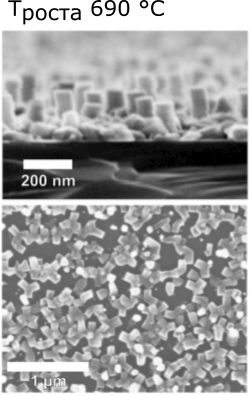
\includegraphics[width=0.25\linewidth]{Image_25_1}}
			\subcaptionbox{\label{fig:Image_25_2}}{%
				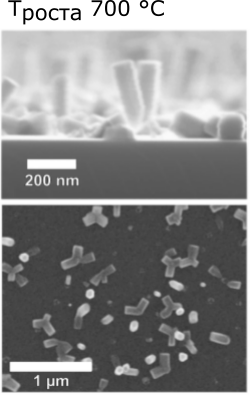
\includegraphics[width=0.25\linewidth]{Image_25_2}}
				\subcaptionbox{\label{fig:Image_25_3}}{%
			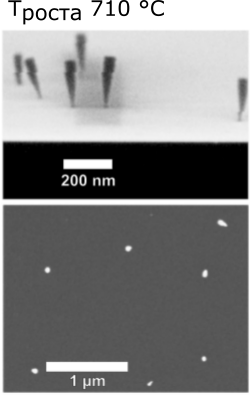
\includegraphics[width=0.25\linewidth]{Image_25_3}} } \legend{Ростовая
		температура: 690~\si{\degreeCelsius}~(а), 700~\si{\degreeCelsius}~(б),
	710~\si{\degreeCelsius}~(в)} \caption{РЭМ изображения (вид сверху и сбоку)
морфологии наноструктур GaN, синтезированных при различных температурах
подложки}\label{fig:Image_25} \end{figure}

\begin{figure}[ht] \centerfloat{ \subcaptionbox{\label{fig:Image_26_1_1}}{%
			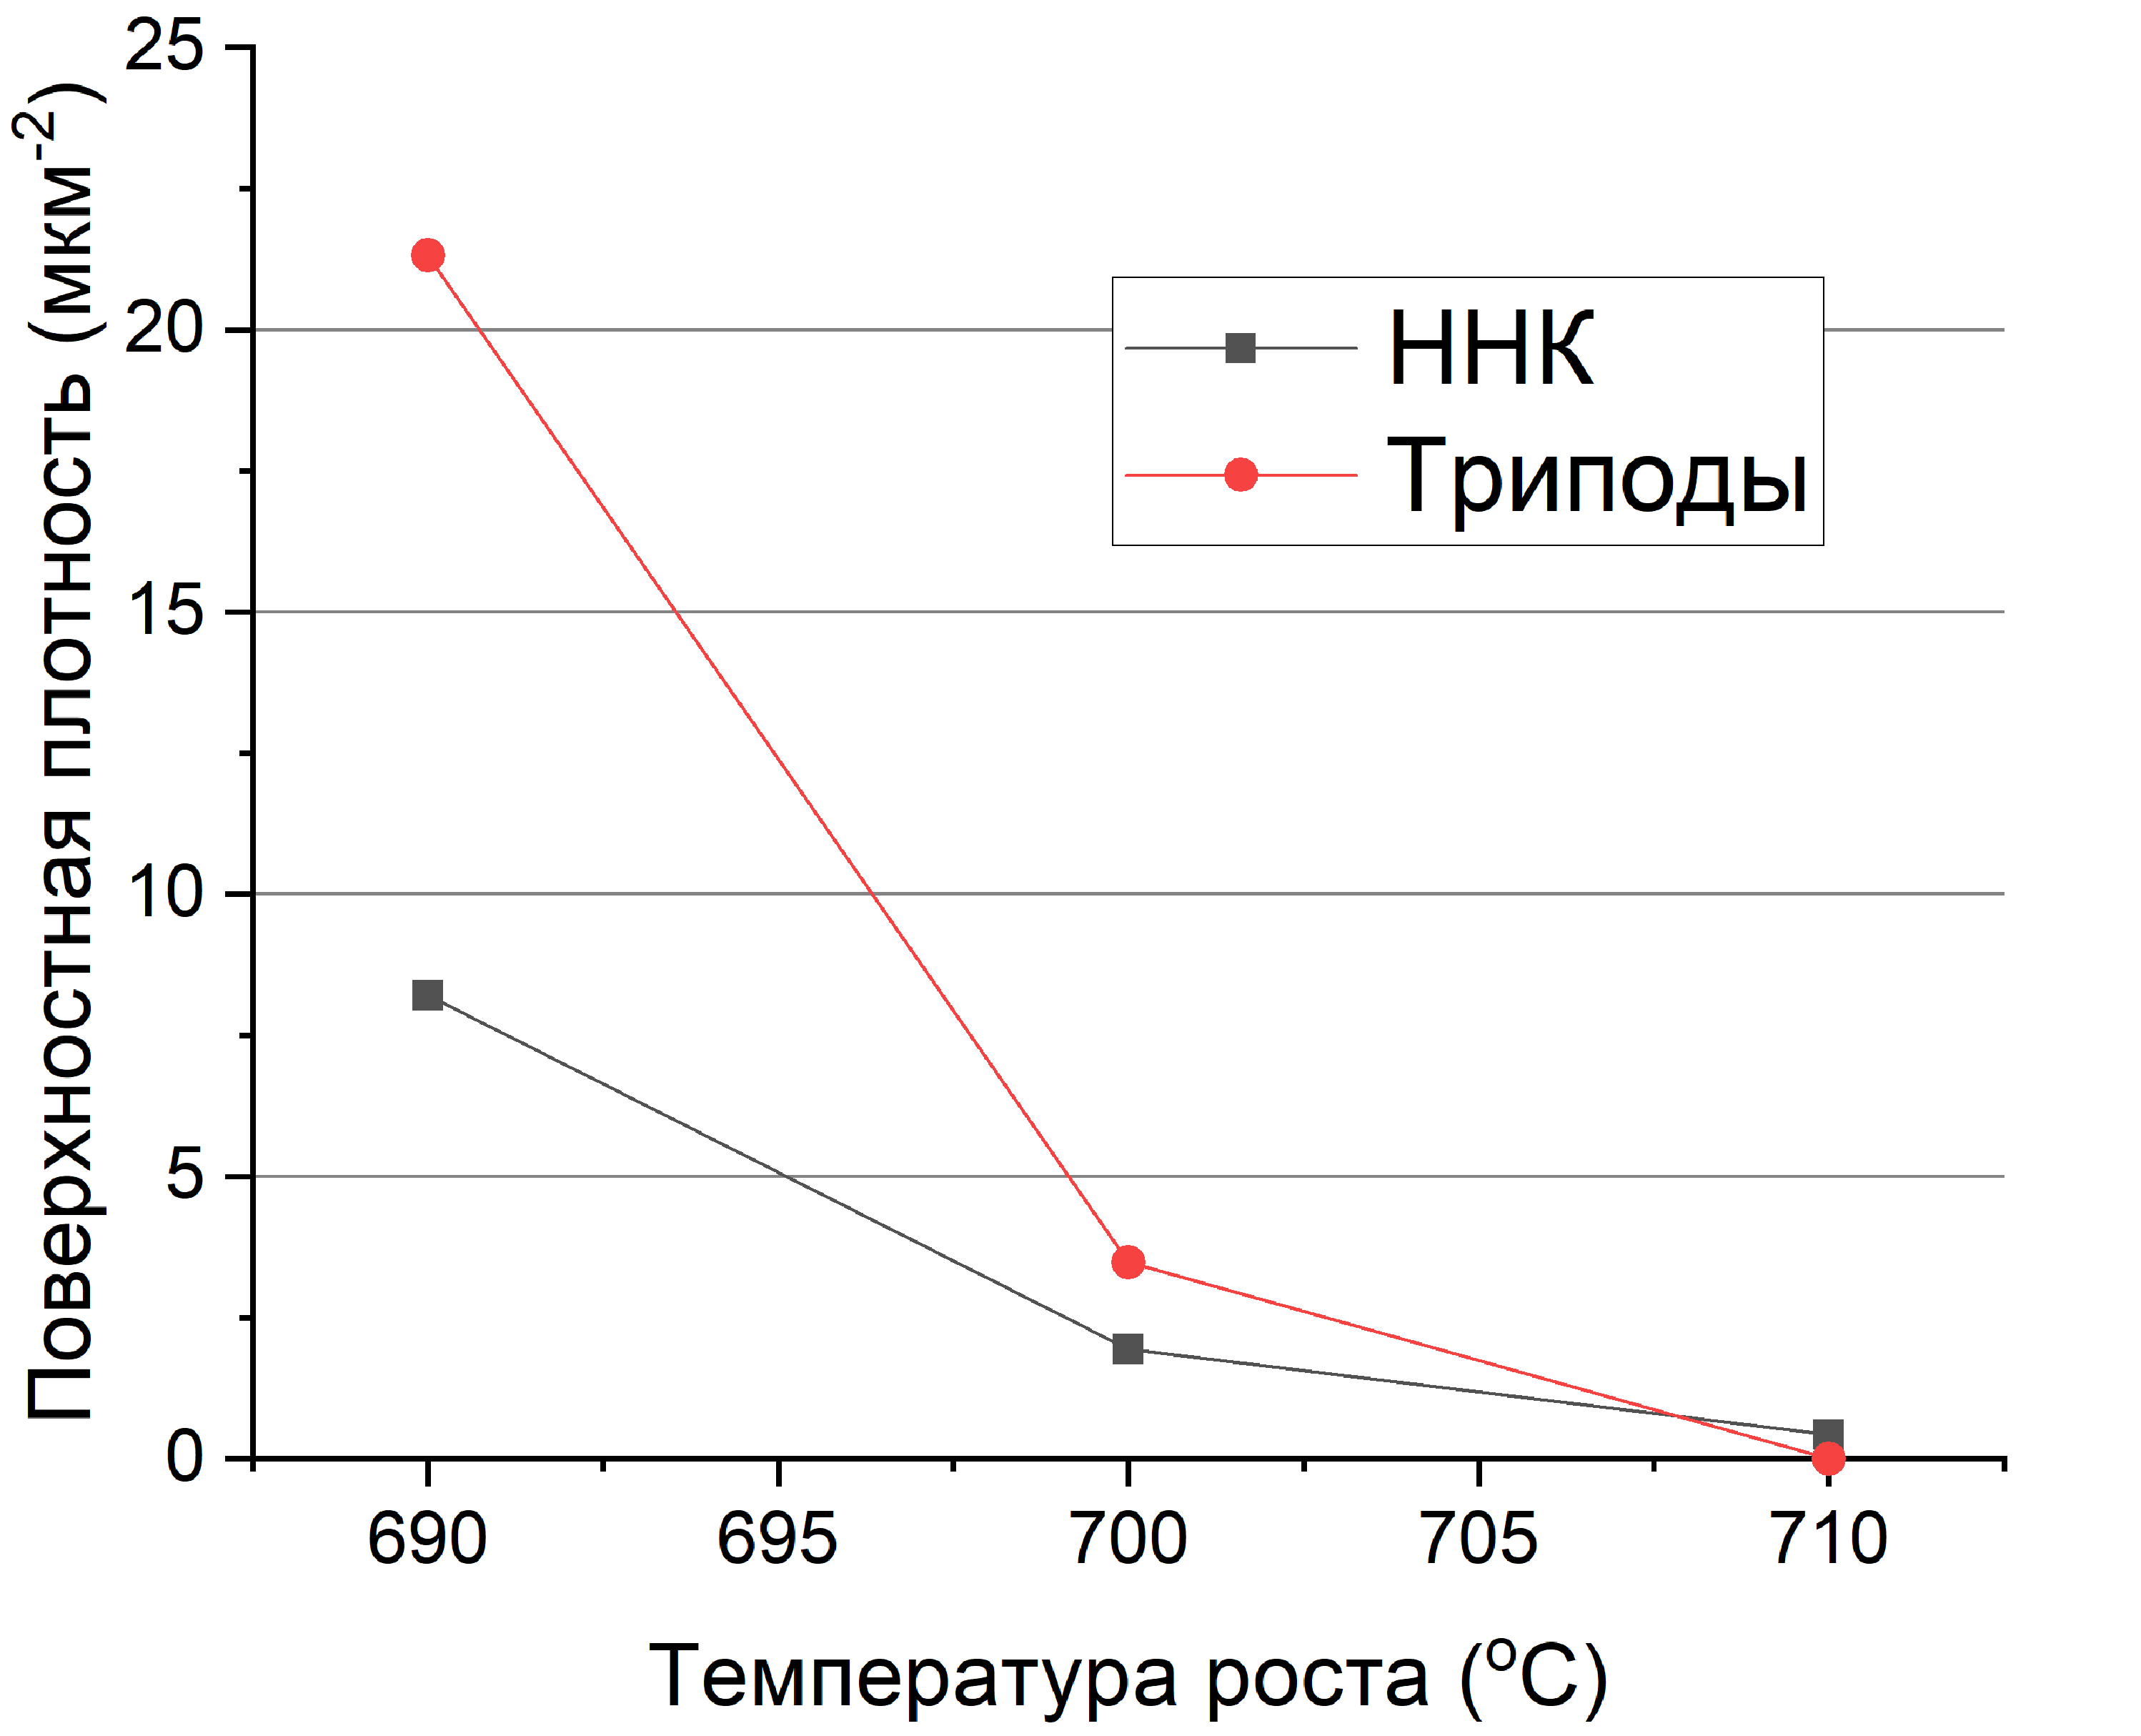
\includegraphics[width=0.48\linewidth]{Image_26_1_1}}
			\subcaptionbox{\label{fig:Image_26_1_2}}{%
		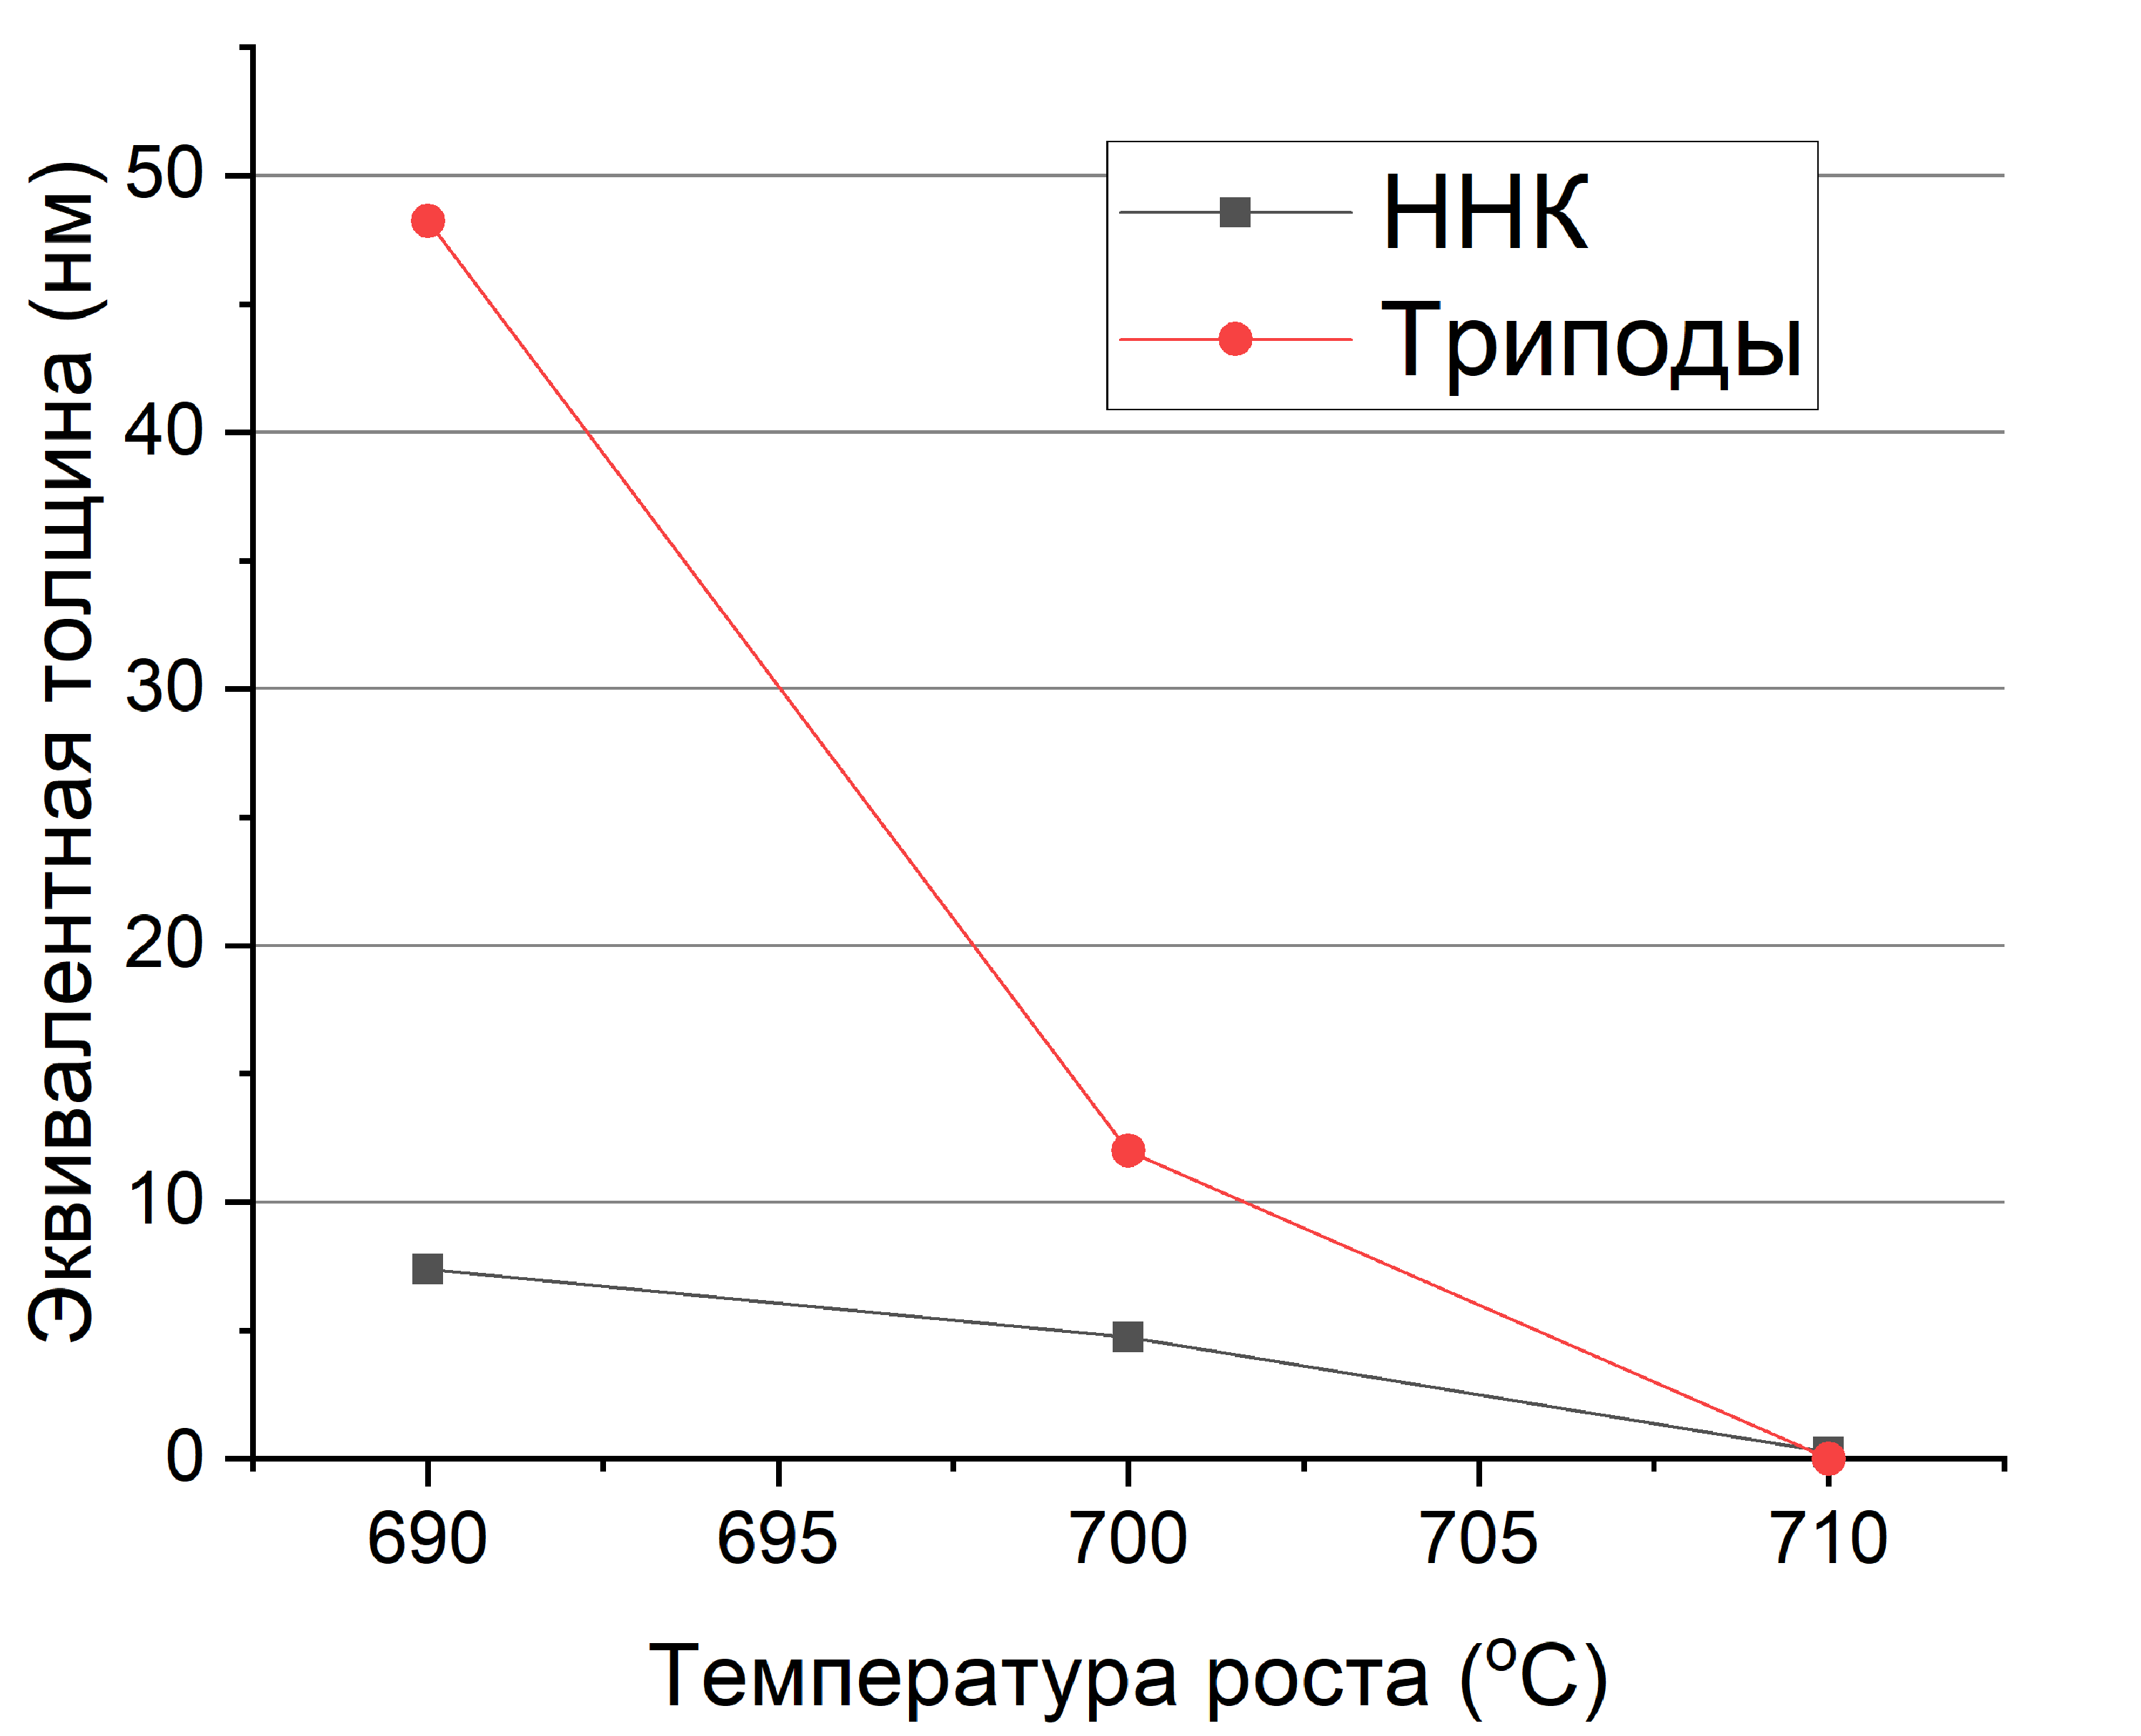
\includegraphics[width=0.48\linewidth]{Image_26_1_2}} }
		\caption{Зависимости поверхностной плотности~(а) и эквивалентной
		толщины~(б) наноструктур GaN от температуры роста}\label{fig:Image_26_1}
	\end{figure}

Эквивалентная толщина синтезированного материала и поверхностная плотность
наноструктур уменьшаются на порядок с повышением температуры с 690 до
710~\si{\degreeCelsius} (см.~рис.~\cref{fig:Image_26_1}). При температуре
700~\si{\degreeCelsius} формируются наиболее длинные ННК и наиболее крупные
триподы (см.~рис.~\cref{fig:Image_26_2}). Повышение температуры роста
увеличивает длину свободного пробега адатомов, что при 700~\si{\degreeCelsius}
приводит к увеличению аксиальной скорости роста. Можно предположить, что
снижение скорости роста наноструктур при дальнейшем повышении температуры
вызвано доминированием десорбции адатомов (см.~рис.~\cref{fig:Image_26_2}).

\begin{figure}[ht] \centerfloat{
	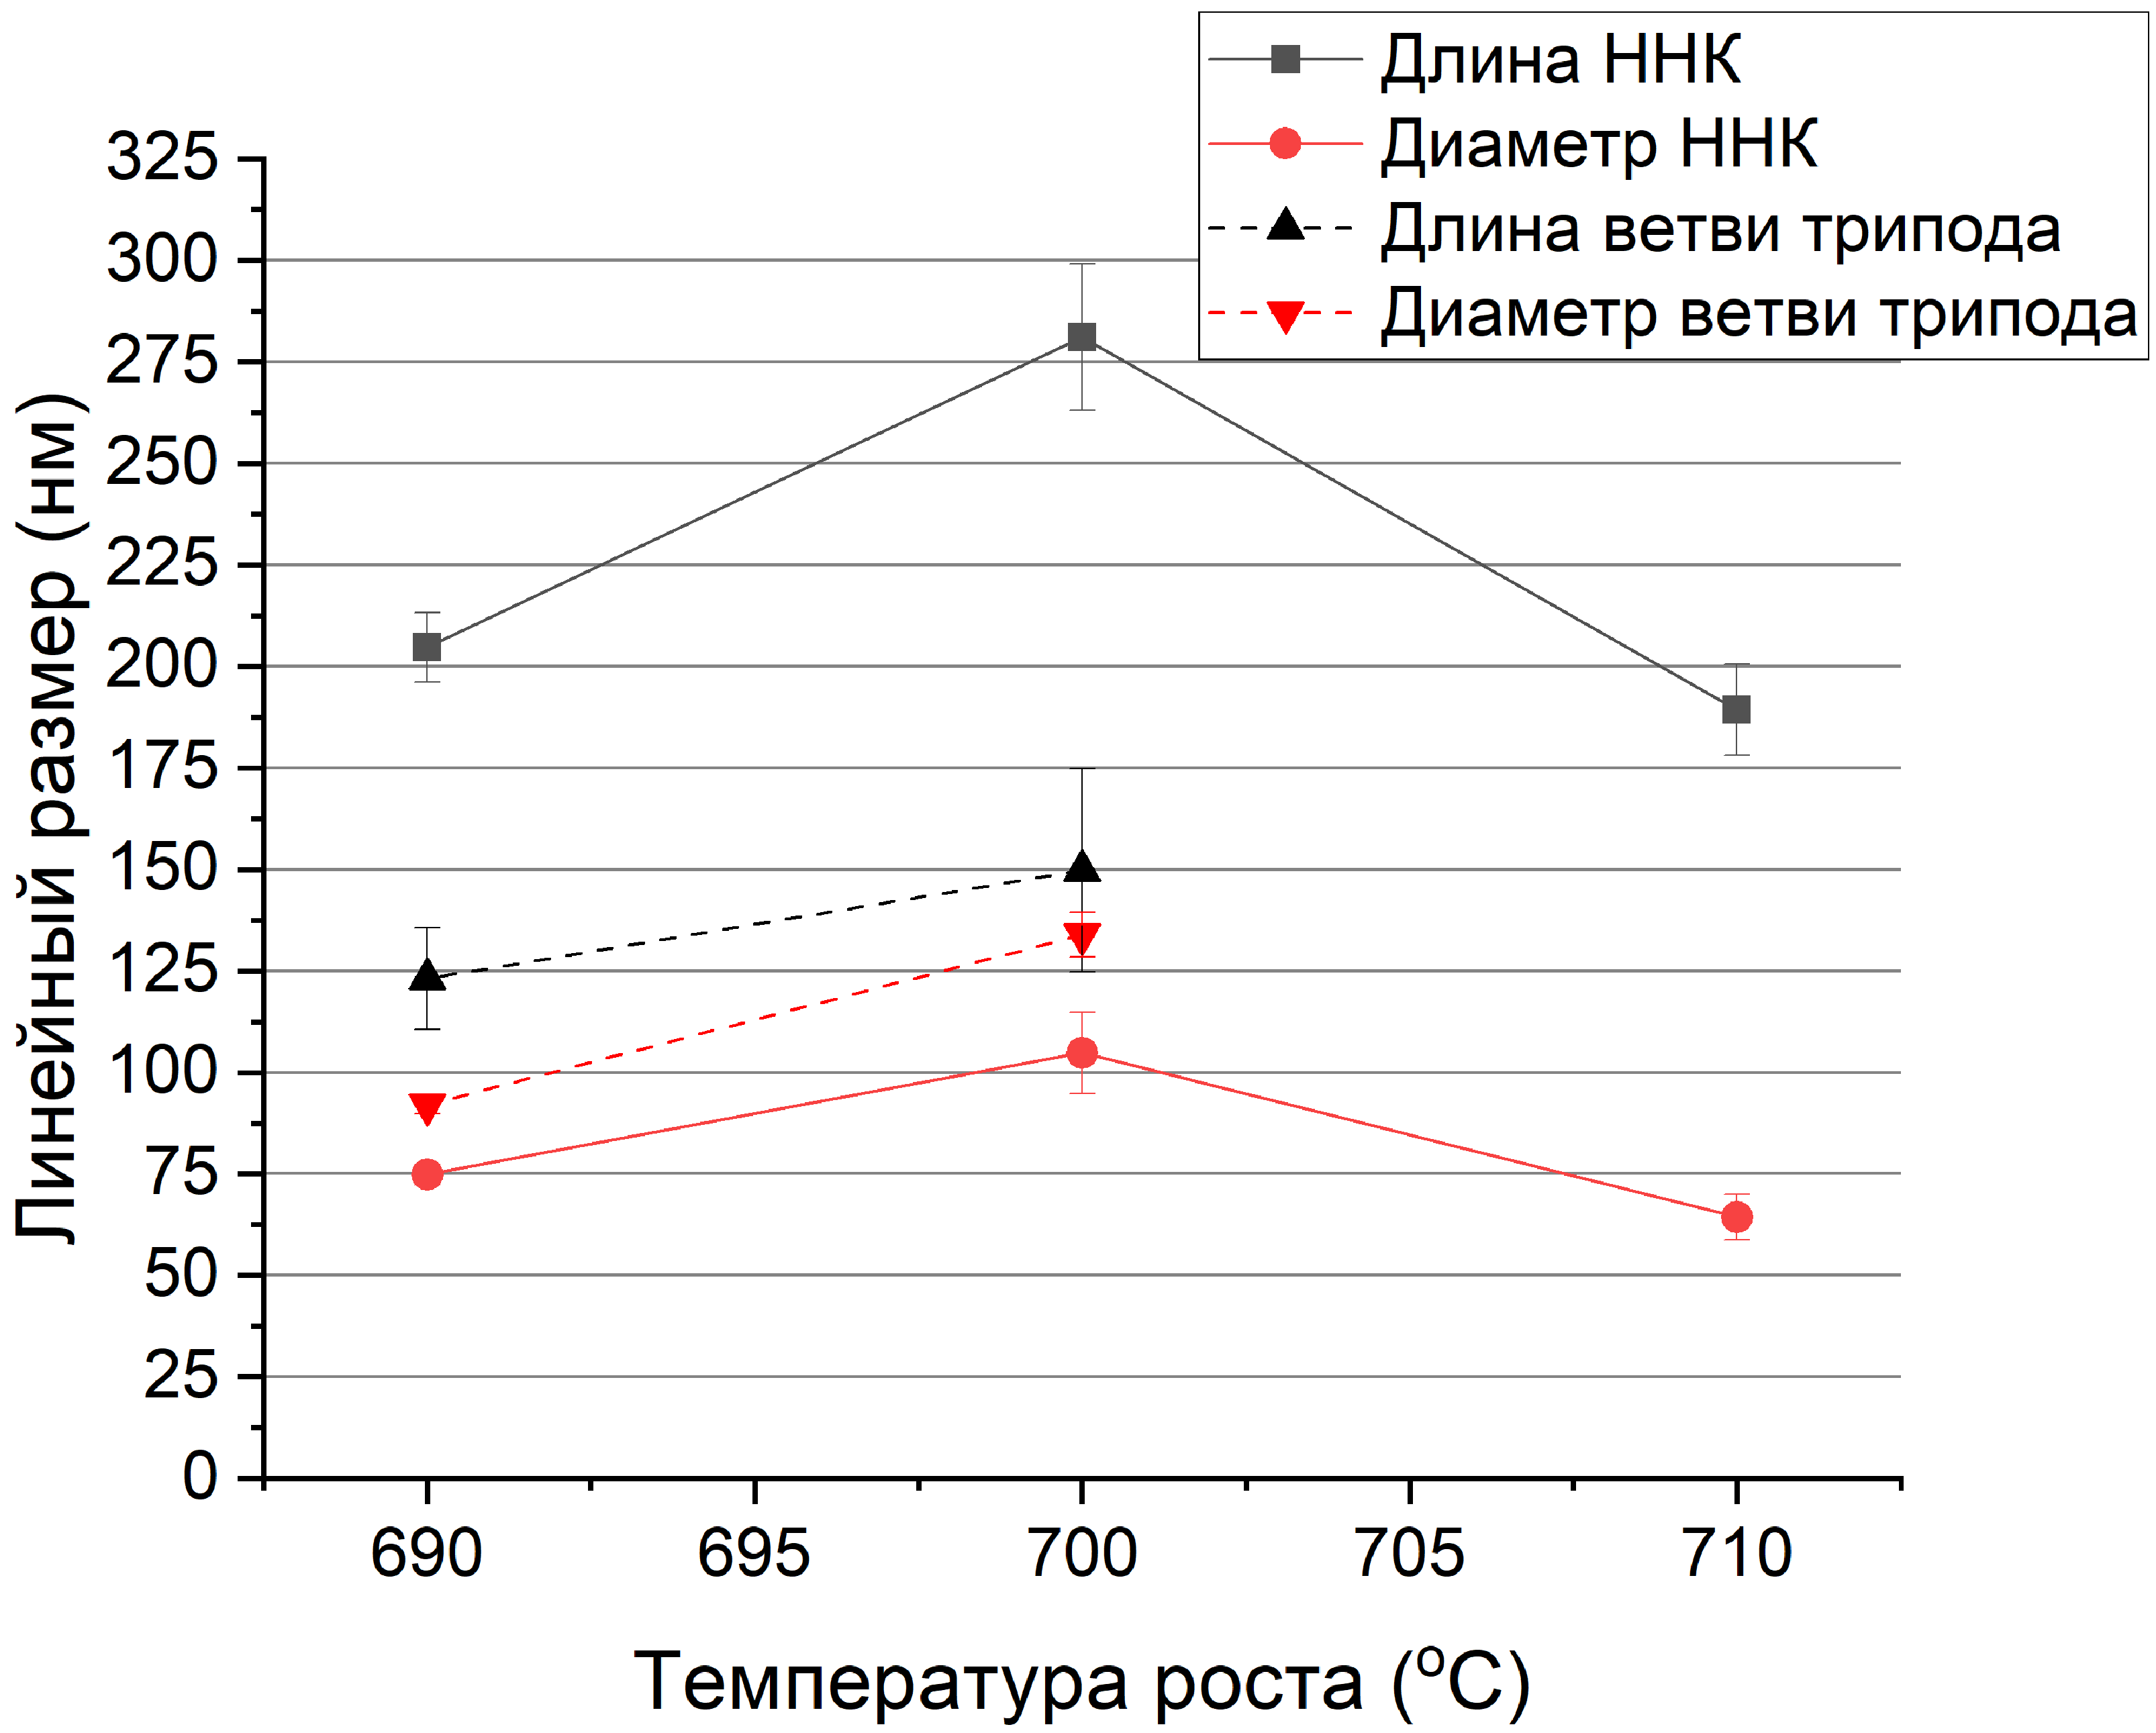
\includegraphics[width=0.6\linewidth]{Image_26_2} } \caption{Зависимости
линейных размеров наноструктур GaN от температуры роста}\label{fig:Image_26_2}
\end{figure}

Основание ННК имеет сужение к подложке. Угол вершины конуса основания ННК
(см.~рис.~\cref{fig:Image_25}) зависит от температуры и времени роста и лежит в
диапазоне от 20{\textdegree} до 42{\textdegree} (\(20\si{\degree} \pm
4\si{\degree}\) при температуре роста 710~\si{\degreeCelsius} и
\(42\si{\degree} \pm 2\si{\degree}\) при температуре роста
700~\si{\degreeCelsius}) \cite{Bolshakov2014}. Морфология ННК может зависеть от
положения подложки относительно источника \cite{Galopin2011}, поскольку оно
влияет на соотношение между молекулярными потоками, попадающими на боковые
стенки и верхнюю грань, таким образом оказывая влияние на длину свободного
пробега до встраивания адатомов Ga на боковых стенках. Это объясняет
зависимость от температуры: если источник азота расположен ортогонально
подложке~--- формируются GaN ННК с однородным по длине диаметром, а если под
острым (как в МПЭ установке Veeco GEN III)~--- ННК с утолщением.

\section{Основные результаты}\label{sec:ch3/sec7}

Продемонстрирован эпитаксиальный синтез методом ПА-МПЭ наноструктур и в форме
GaN ННК и триподов на Si(111) подложке с предварительным формированием
затравочных наноостровков GaN. После нитридации наноостровки приобретают
кольцеобразную форму. Данные островки имеют ZB структуру и впоследствии
находятся в основе триподов и наклоненных ННК.

Поверхностная плотность, размер и аспектное отношение структур можно
контролировать температурой роста, потоком III группы и эквивалентной толщиной
затравочного слоя. Нуклеация триподов может быть полностью подавлена путем
уменьшения эквивалентной толщины затравки Ga и повышения температуры роста выше
710~\si{\degreeCelsius}.

Направление ветвей соответствует кристаллографическому направлению
<\(0001\)>\textsubscript{GaN} с преимущественной ориентацией вдоль направлений
<\(1\overline{1}0\)>\textsubscript{Si}, <\(11\overline{2}\)>\textsubscript{Si}
и \(<12\overline{3}>\)\textsubscript{Si}. Плоскость
\((11\overline{2}1)\)\textsubscript{GaN} триподов имеет эпитаксиальное
отношение с параллельной плоскостью подложки (111)\textsubscript{Si}.

Спектр ФЛ от массив нанотриподов с включениями политипа ZB имеет три полосы:
интенсивную полосу, характерную для объемного WZ GaN (\(\approx
3,48\)~\si{\electronvolt}), полосу, характерную для GaN с дефектами упаковки
(\(\approx 3,43\)~\si{\electronvolt}) и полосу, характерную для ZB GaN
(\(\approx 3,25\)~\si{\electronvolt}).

\FloatBarrier
